\section{Numerical Methods -- Integrals, Derivatives, and Newton's Method}
\subsection{Numerical Integration of Functions}
Numerical integration is the numerical approximation of
\begin{equation}
I = \int_a^b f(x)dx
\end{equation}
 
Consider the problem of determining the shaded area under the curve $y = f(x)$ from $x = a$ to $x = b$, as depicted in Figure \ref{fig:IntegrationPanels}, and suppose that analytical integration is not feasible. 
 
\begin{figure}[h!] %  figure placement: here, top, bottom, or page
   \centering
   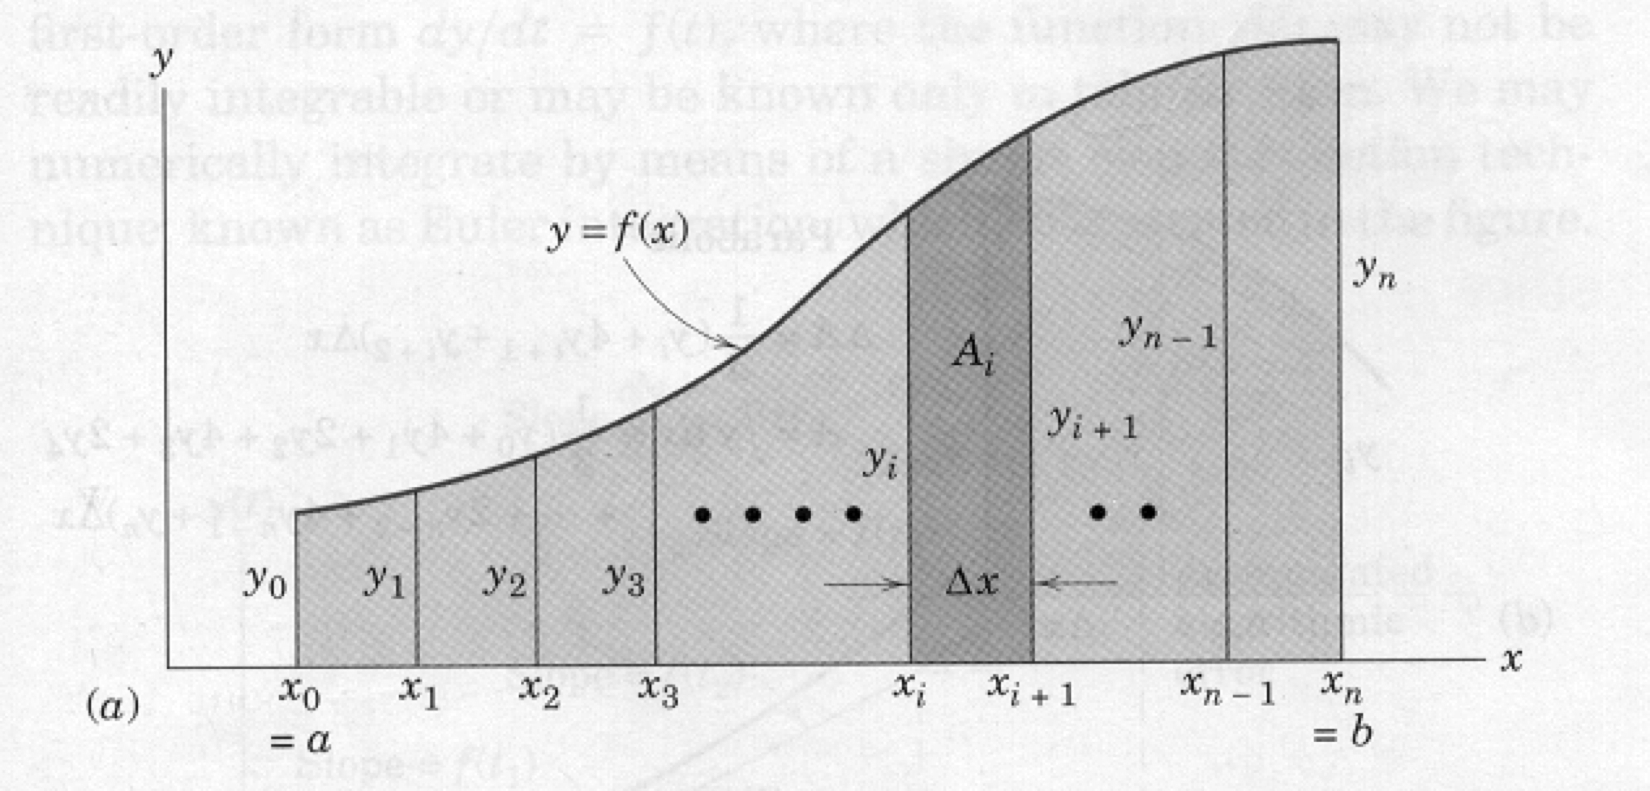
\includegraphics[width=5in]{./3-Differentation/IntegrationPanels.jpg} 
   \caption{Schematic of Panels for Numerical Integration. }
   \label{fig:IntegrationPanels}
\end{figure}

The function may be known in tabular form from experimental measurements or it may be known in an analytical form. 
The function is taken to be continuous within the interval $a < x < b$. 
We may divide the area into $n$ vertical panels, each of width $\Delta x = (b - a)/n$, and then add the areas of all strips to obtain  $A~\approx \int ydx$.

A representative panel of area $A_i$ is shown with darker shading in the figure. 
Three useful numerical approximations are listed in the following sections.    
The approximations differ in how the function is represented by the panels --- in all cases the function is approximated by known polynomial models between the panel end points.

In each case the greater the number of strips, and correspondingly smaller value of $\Delta x$, the more accurate the approximation. 
Typically, one can begin with a relatively small number of panels and increase the number until the resulting area approximation stops changing.

\subsubsection{Rectangular Panels}
Figure \ref{fig:RectangularPanels} is a schematic of a rectangular panels.  The figure is assuming the function structure is known and can be evaluated at an arbitrary location in the $\Delta x$ dimension.  
\begin{figure}[h!] %  figure placement: here, top, bottom, or page
   \centering
   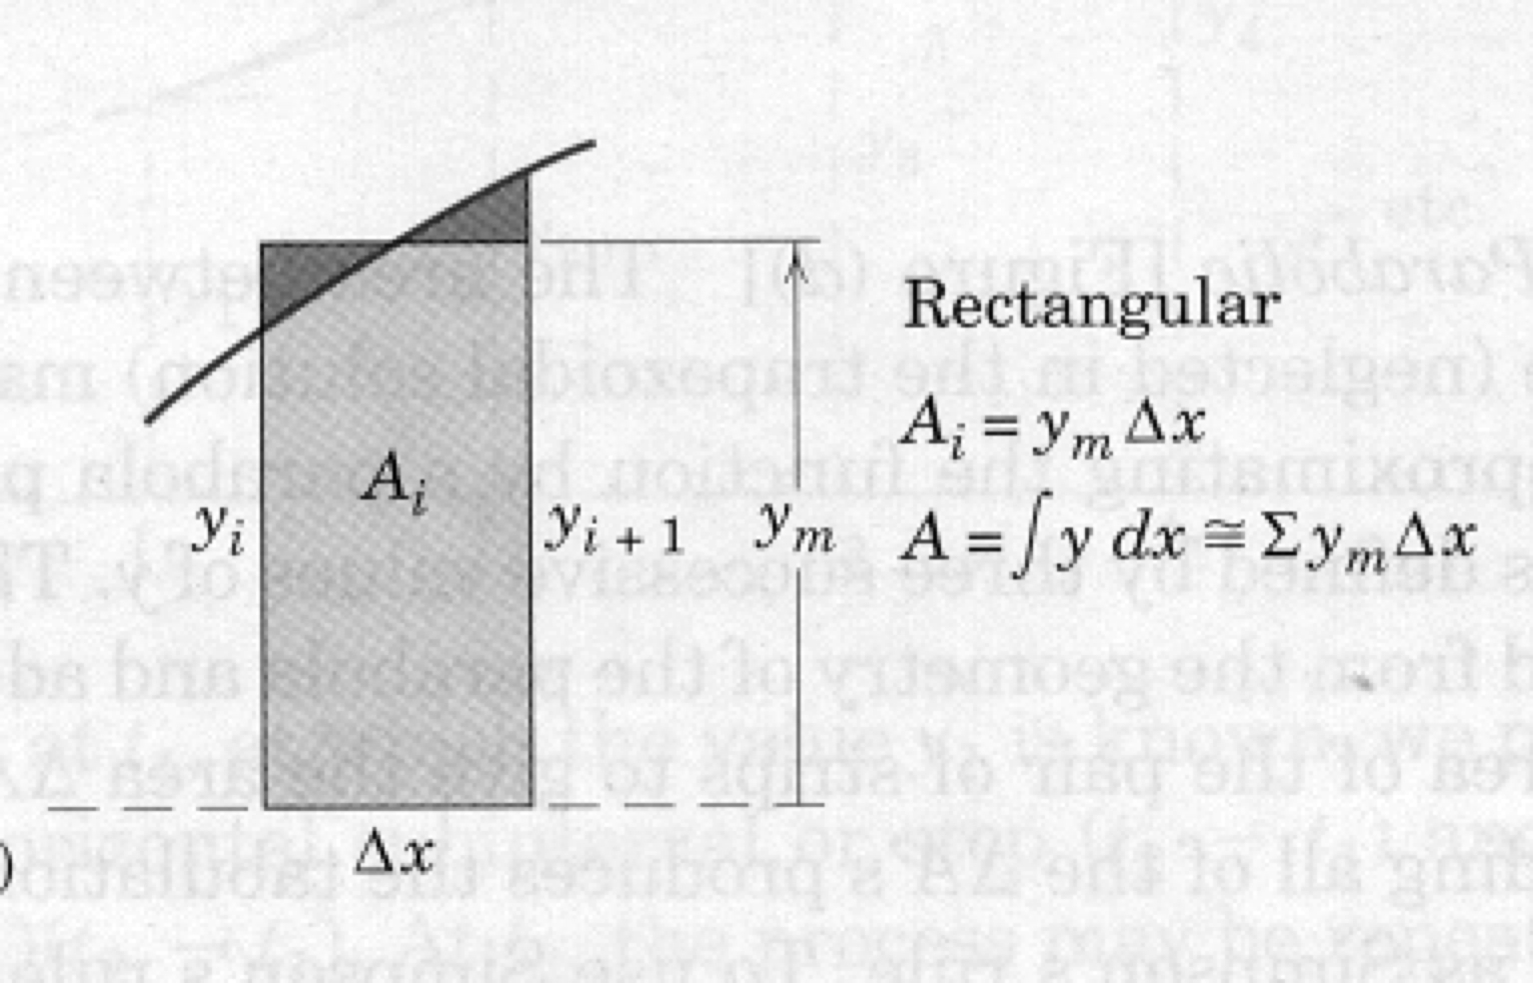
\includegraphics[width=5in]{./3-Differentation/RectangularPanels.jpg} 
   \caption{Rectangular Panel Schematic.}
   \label{fig:RectangularPanels}
\end{figure}
Each panels is treated as a rectangle, as shown by the representative panel whose height $y_m$ is chosen visually so that the small cross-hatched areas are as nearly equal as possible. Thus, we form the sum $\sum y_m$ of the effective heights and multiply by $\Delta x$. For a function known in analytical form, a value for $y_m$ equal to that of the function at the midpoint $x_i + \Delta x /2$ may be calculated and used in the summation.

For tabulated functions, we have to choose to either take $y_m$ as the value at the left endpoint or right endpoint.    This limitation is often quite handy when we are trying to integrate a function that is integrable, but undefined on one endpoint.

Lets try some examples in \textbf{R}.\\

\newpage \textbf{Problem:} Find the area under the curve $y= x\sqrt{1+x^2}$  from $x = 0$ to $x = 2$.

\textbf{Solution:} One solution is shown in Figure \ref{fig:RectExample},which is a screen capture of a rudimentary code that implements the rectangular panel method.\footnote{The exact solution is A=3.393477}   
\begin{figure}[h!] %  figure placement: here, top, bottom, or page
   \centering
   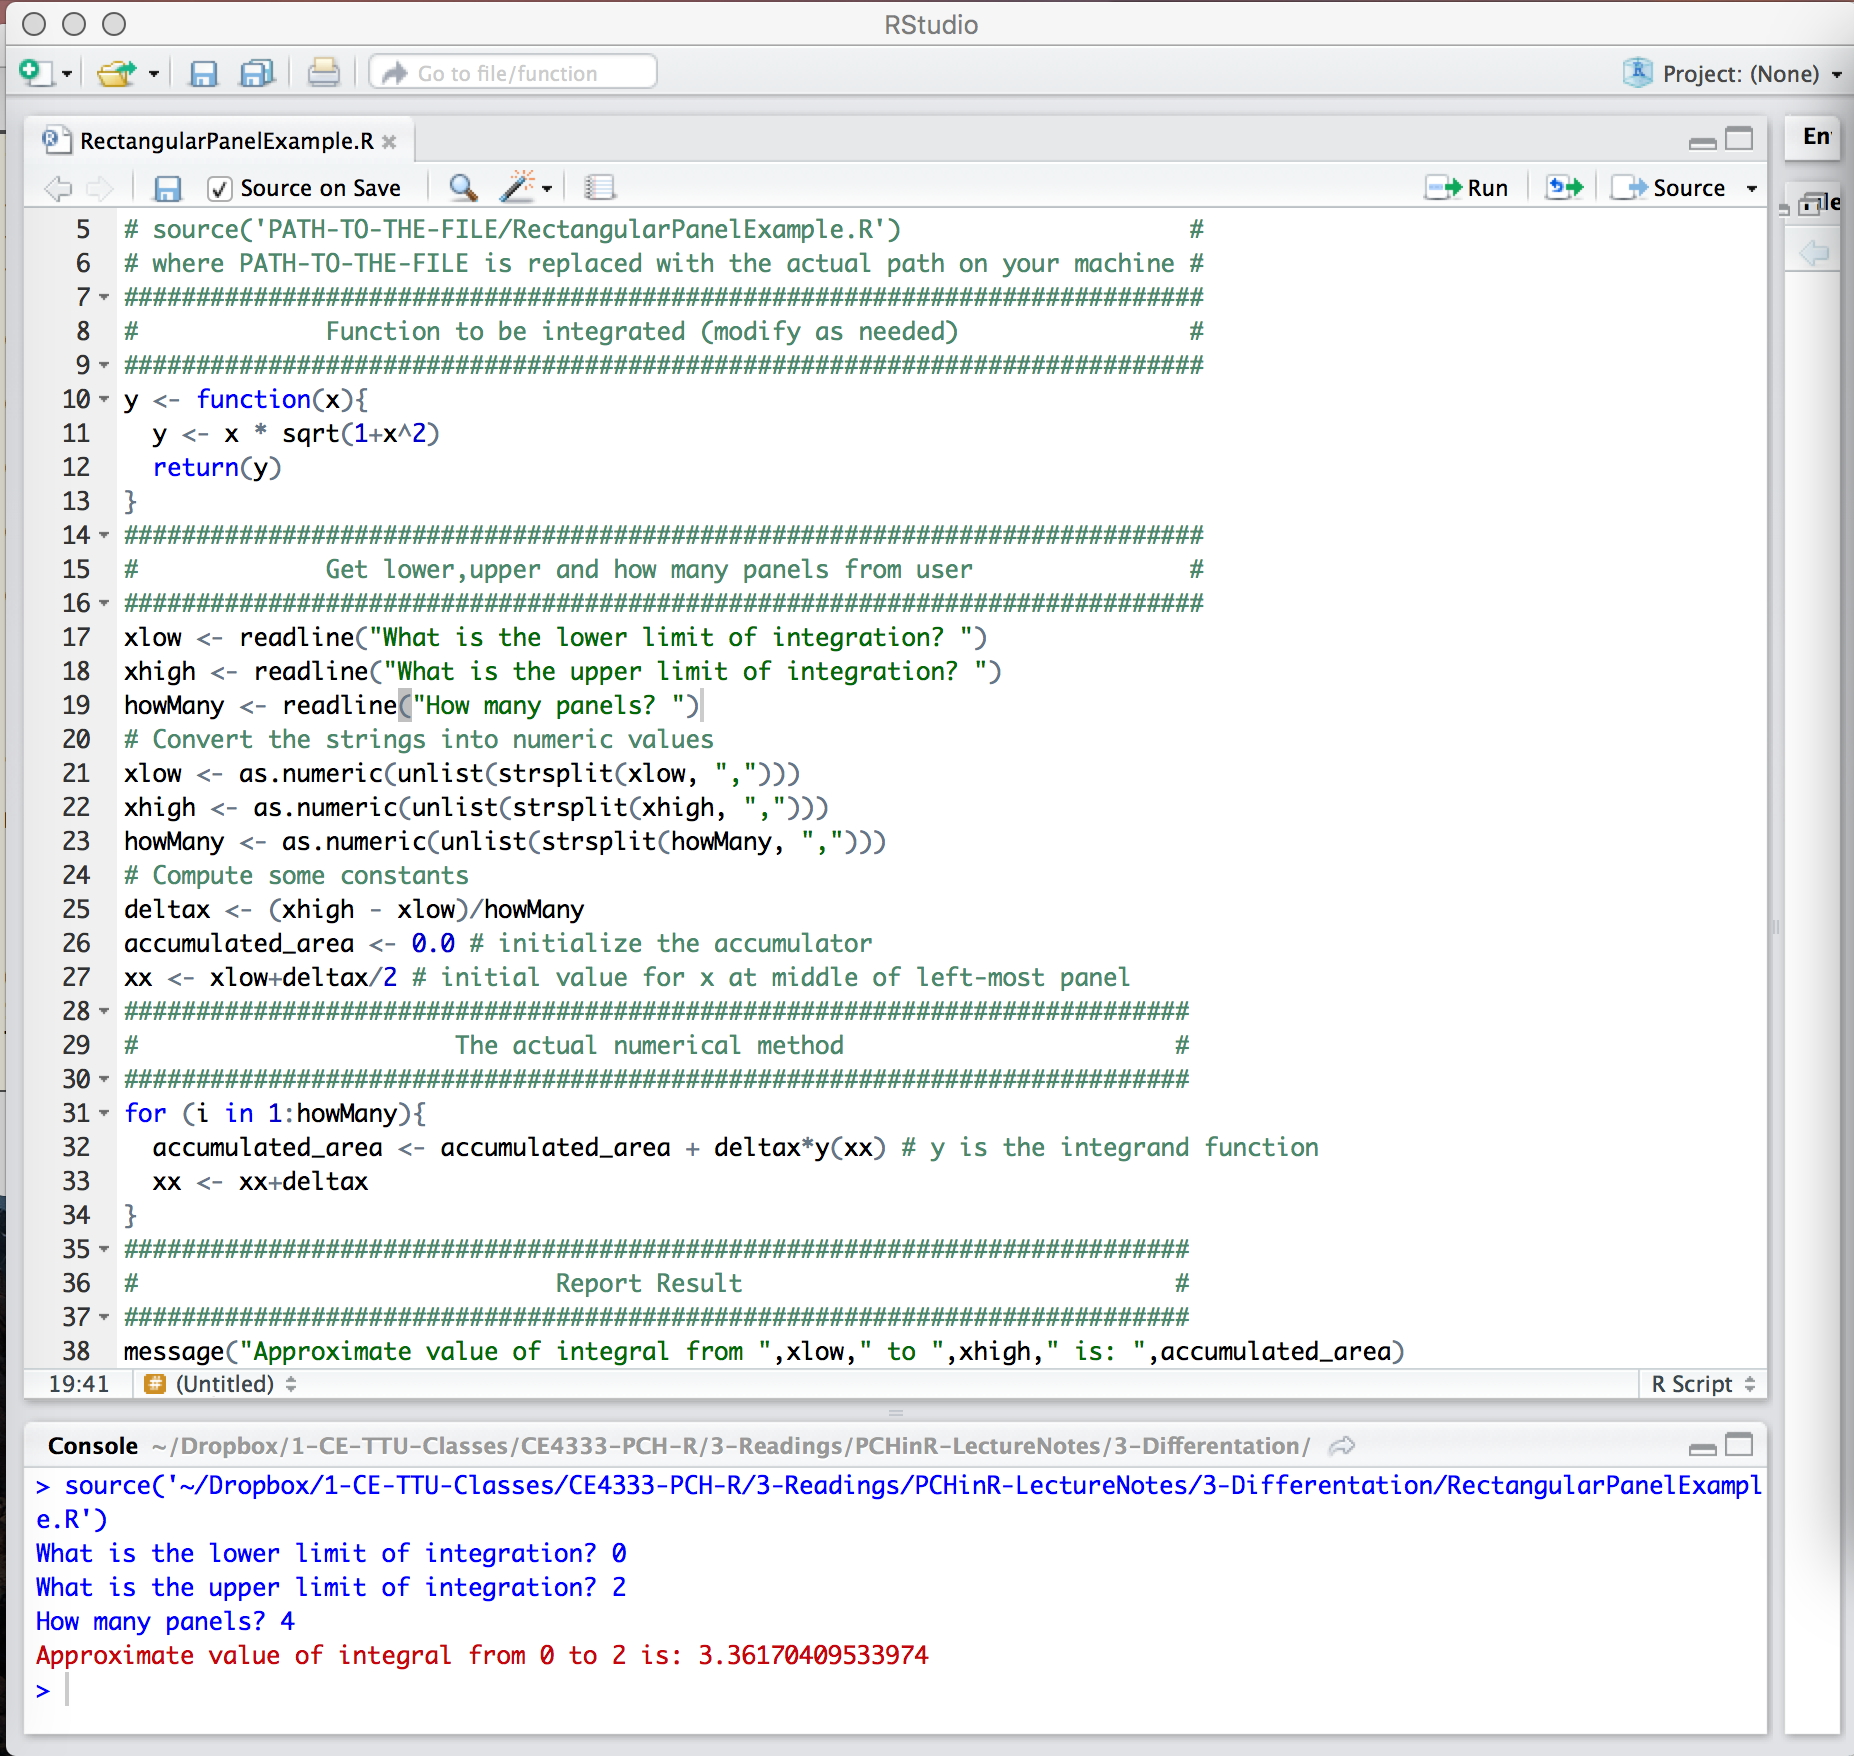
\includegraphics[width=6in]{./3-Differentation/RectExample.jpg} 
   \caption{Rectangular panel example showing code and resulting computed area using just 4 panels.}
   \label{fig:RectExample}
\end{figure}

The script does not implement any kind of error checking -- we could enter text values for the lower and upper values of $x$ as well as the number of panels to use, and the script would attempt to run. 
A better version would force us to enter numeric values, and check for undefined ranges and such; devotion to error trapping is typical for professional programs where you are going to distribute executable modules and not expect the end user to be a programmer.

For the time being, we will accept this approach (error trapping is left as an exercise), however in your own scripts you should implement error traps where possible -- you may start without them but as you maintain your scripts, you will learn where data entry errors occur and trap them.\footnote{For example, traps are used to force the user to enter a value that actually is meaningful, or select a default value, or internally prevent division by zero.}

The actual listing depicted in Figure \ref{fig:RectExample} is shown in Listing \ref{lst:RectPanels}

\begin{lstlisting}[caption=R code demonstrating Rectangular Panel Numerical Integration, label=lst:RectPanels]
# R script to implement rectangular panel numerical integration
################################# NOTE ####################################
## The interactive input requires the script to be sourced                #
# In R console the command line would be                                  #
# source('PATH-TO-THE-FILE/RectangularPanelExample.R')                    #
# where PATH-TO-THE-FILE is replaced with the actual path on your machine #
###########################################################################
#             Function to be integrated (modify as needed)                #
###########################################################################
y <- function(x){
  y <- x * sqrt(1+x^2)
  return(y)
}
###########################################################################
#             Get lower,upper and how many panels from user               #
###########################################################################
xlow <- readline("What is the lower limit of integration? ")  
xhigh <- readline("What is the upper limit of integration? ")
howMany <- readline("How many panels? ")
# Convert the strings into numeric values
xlow <- as.numeric(unlist(strsplit(xlow, ",")))
xhigh <- as.numeric(unlist(strsplit(xhigh, ",")))
howMany <- as.numeric(unlist(strsplit(howMany, ",")))
# Compute some constants
deltax <- (xhigh - xlow)/howMany  
accumulated_area <- 0.0 # initialize the accumulator
xx <- xlow+deltax/2 # initial value for x at middle of left-most panel
##########################################################################
#                      The actual numerical method                       #
##########################################################################
for (i in 1:howMany){
  accumulated_area <- accumulated_area + deltax*y(xx) # y is the integrand function
  xx <- xx+deltax
}
##########################################################################
#                             Report Result                              #
##########################################################################
message("Approximate value of integral from ",xlow," to ",xhigh," is: ",accumulated_area)
\end{lstlisting}

\begin{figure}[h!] %  figure placement: here, top, bottom, or page
   \centering
   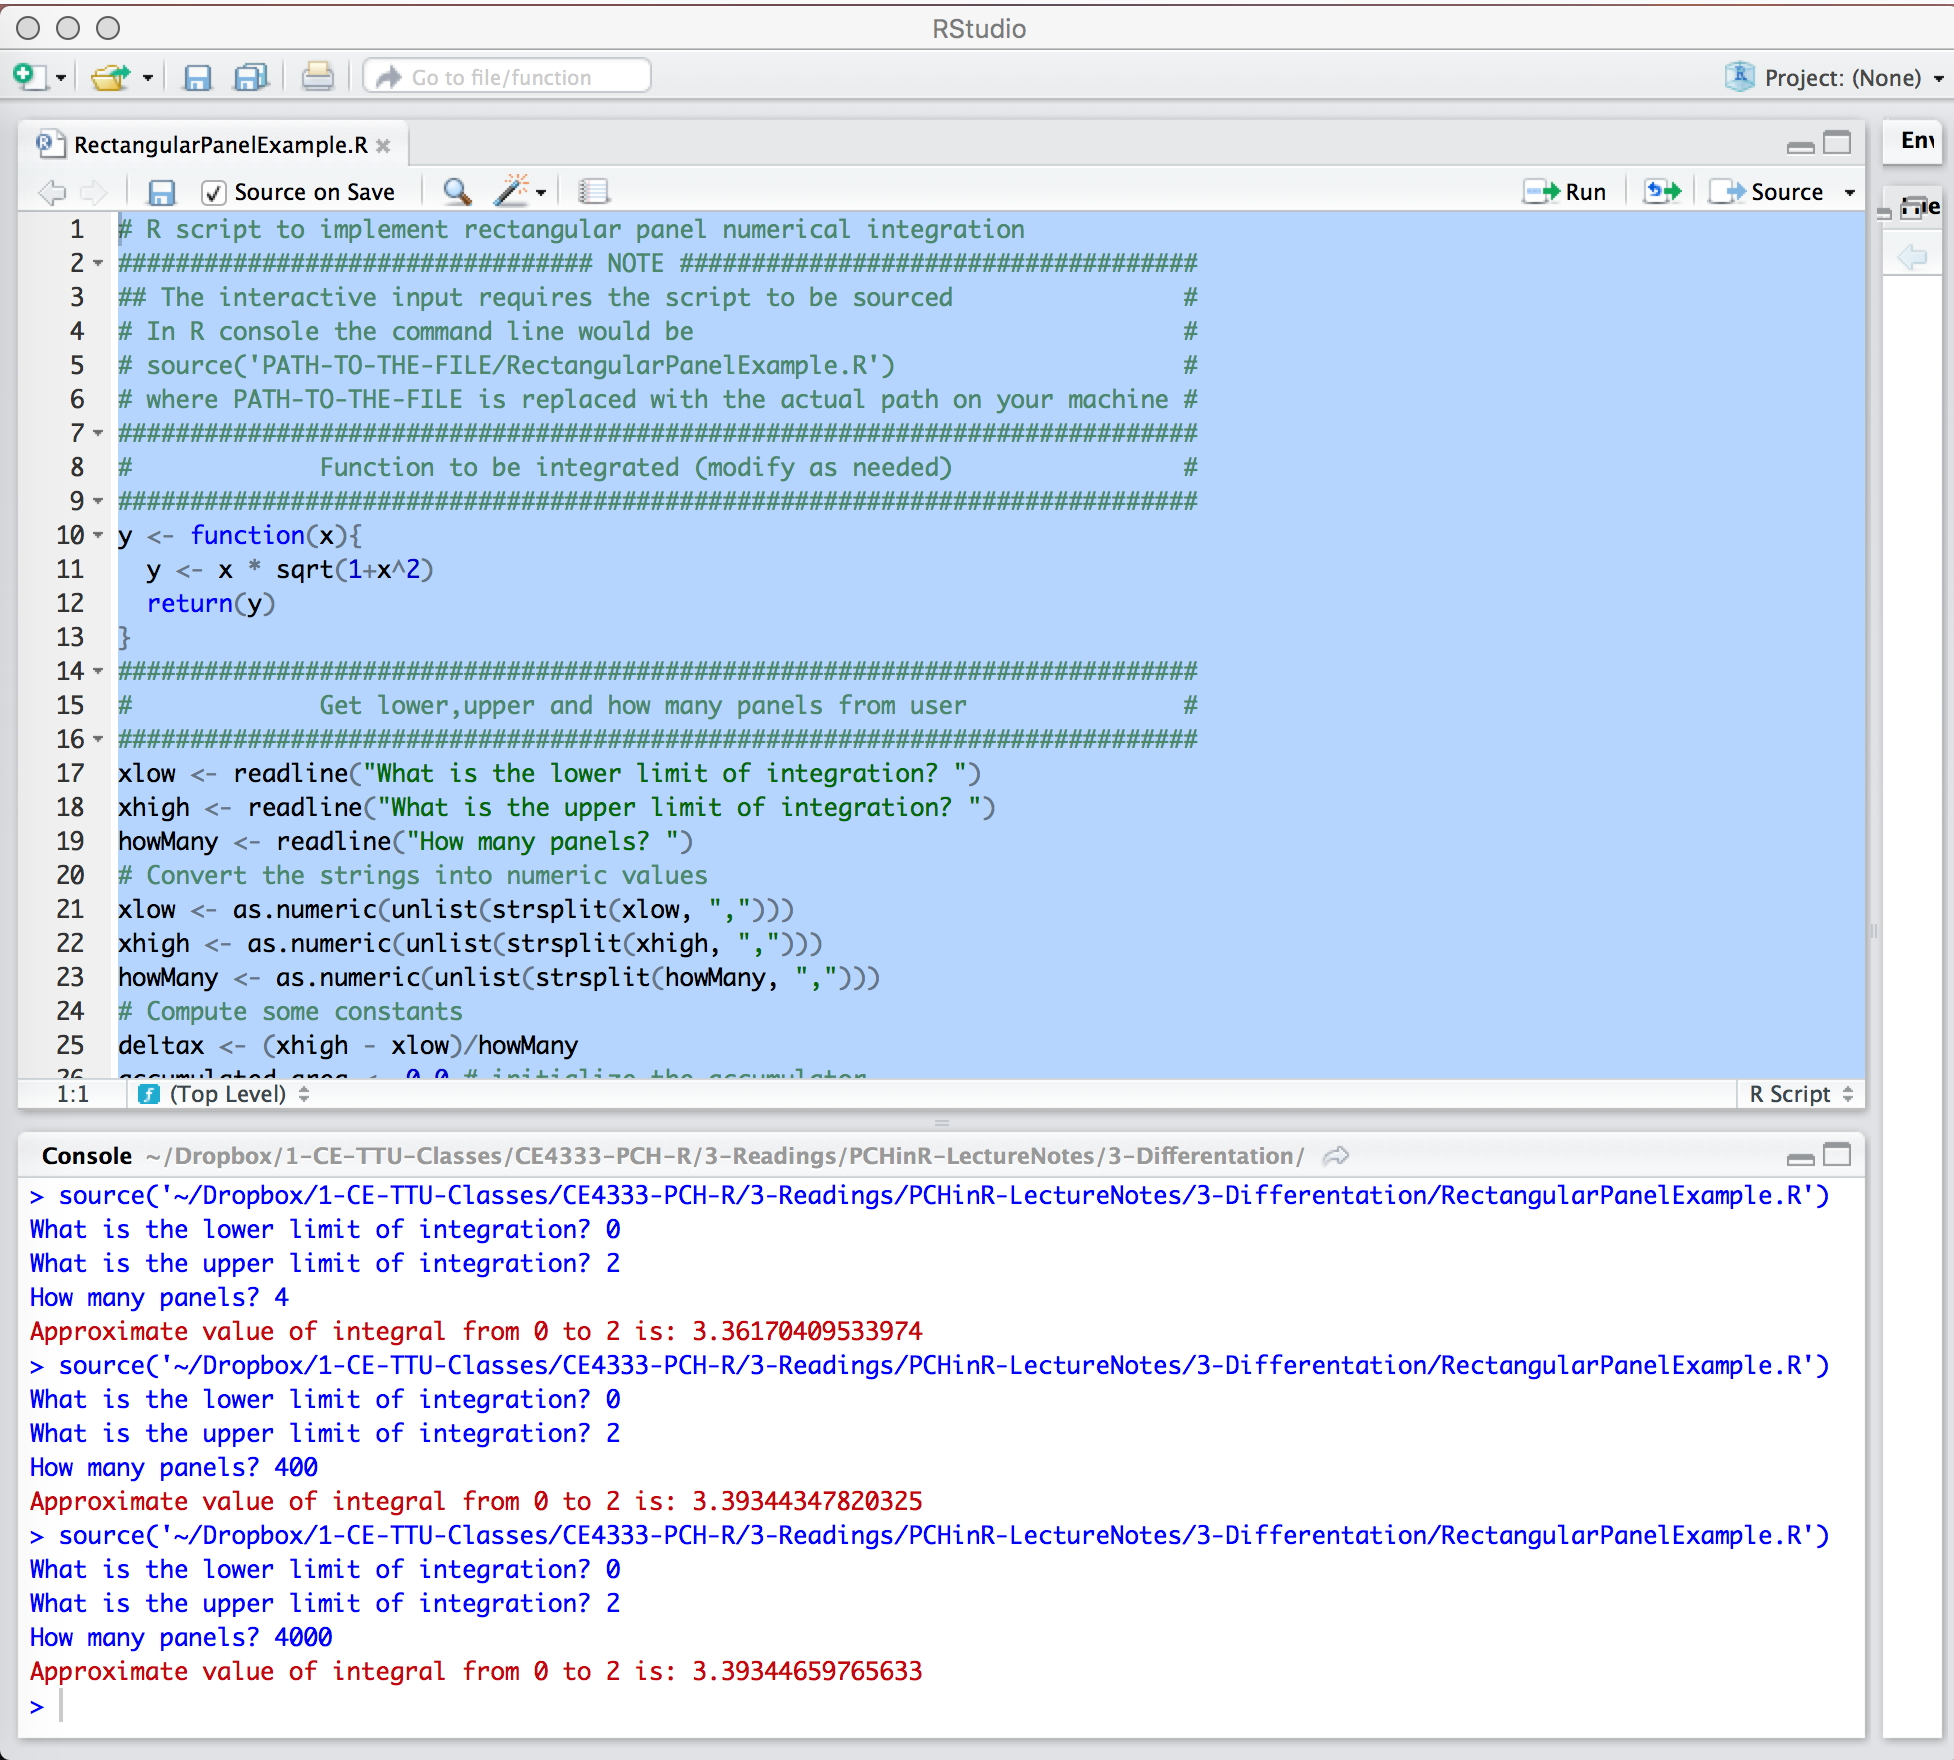
\includegraphics[width=6in]{./3-Differentation/RectExample44.jpg} 
   \caption{Rectangular panel example showing difference in computed area using 4, 400, and 4000 panels.  The 4000 panel result is essentially equivalent to the exact solution.  Such convergence to exact values is typical}
   \label{fig:RectExample44}
\end{figure}
Figure \ref{fig:RectExample44} is the same program run using 4,400, and 4000 panels observe the difference in computed area as well as the results closeness to the exact solution.

\subsubsection{Trapezoidal Panels}
The trapezoidal panels are approximated as shown in Figure \ref{fig:TrapPanels}. The area $A_i$ is the average height $(y_i + y_{i+1} )/2$ times $\Delta x$. Adding the areas gives the area approximation as tabulated.   For the example with the curvature shown, the approximation will be on the low side. For the reverse curvature, the approximation will be on the high side.  The trapezoidal approximation is commonly used with tabulated values.

\begin{figure}[h!] %  figure placement: here, top, bottom, or page
   \centering
   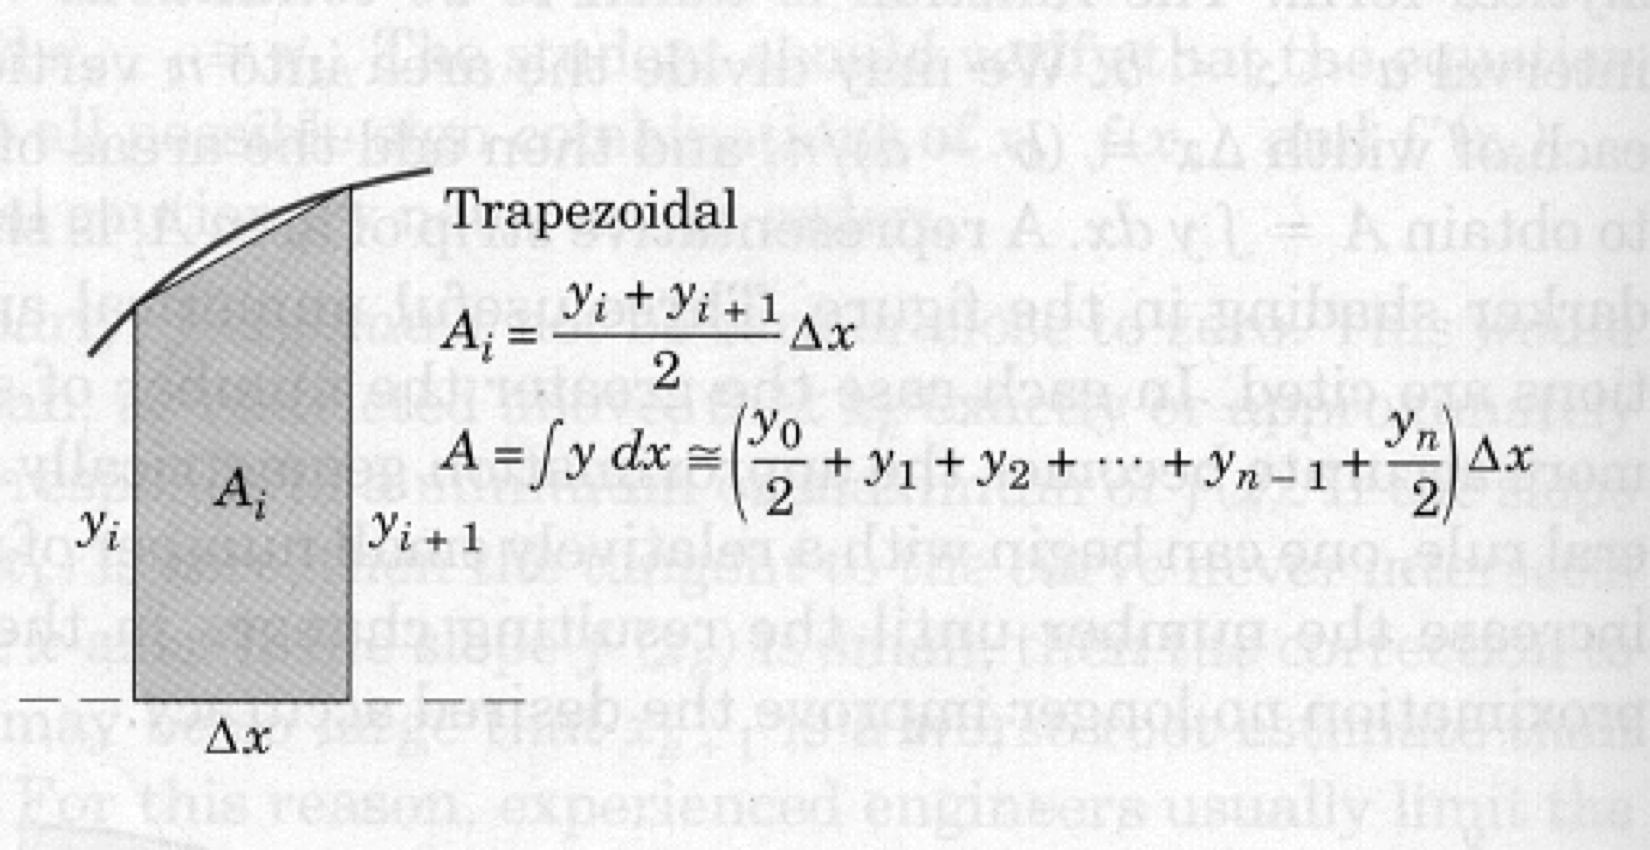
\includegraphics[width=4.3in]{./3-Differentation/TrapPanels.jpg} 
   \caption{Trapezoidal Panel Schematic.}
   \label{fig:TrapPanels}
\end{figure}

The same example as presented for rectangular panels is repeated, except using trapezoidal panels.  The code is changed because we will evaluate at each end of the panel (so no fussing to find an intermediate estimate for where to evaluate the function).

Figure \ref{fig:TrapExample} illustrates the trapezoidal method for approximating an integral.   In the example, the left and right panel endpoints in $x$ are set as separate variables $x_{left}$ and $x_{right}$ and incremented by $\Delta x$ as we step through the count-controlled repetition to accumulate the area.  The corresponding $y$ values are computed within the loop and averaged, then multiplied by $\Delta x$ and added to the accumulator.  Finally the $x$ values are incremented.
 
\begin{figure}[h!] %  figure placement: here, top, bottom, or page
   \centering
   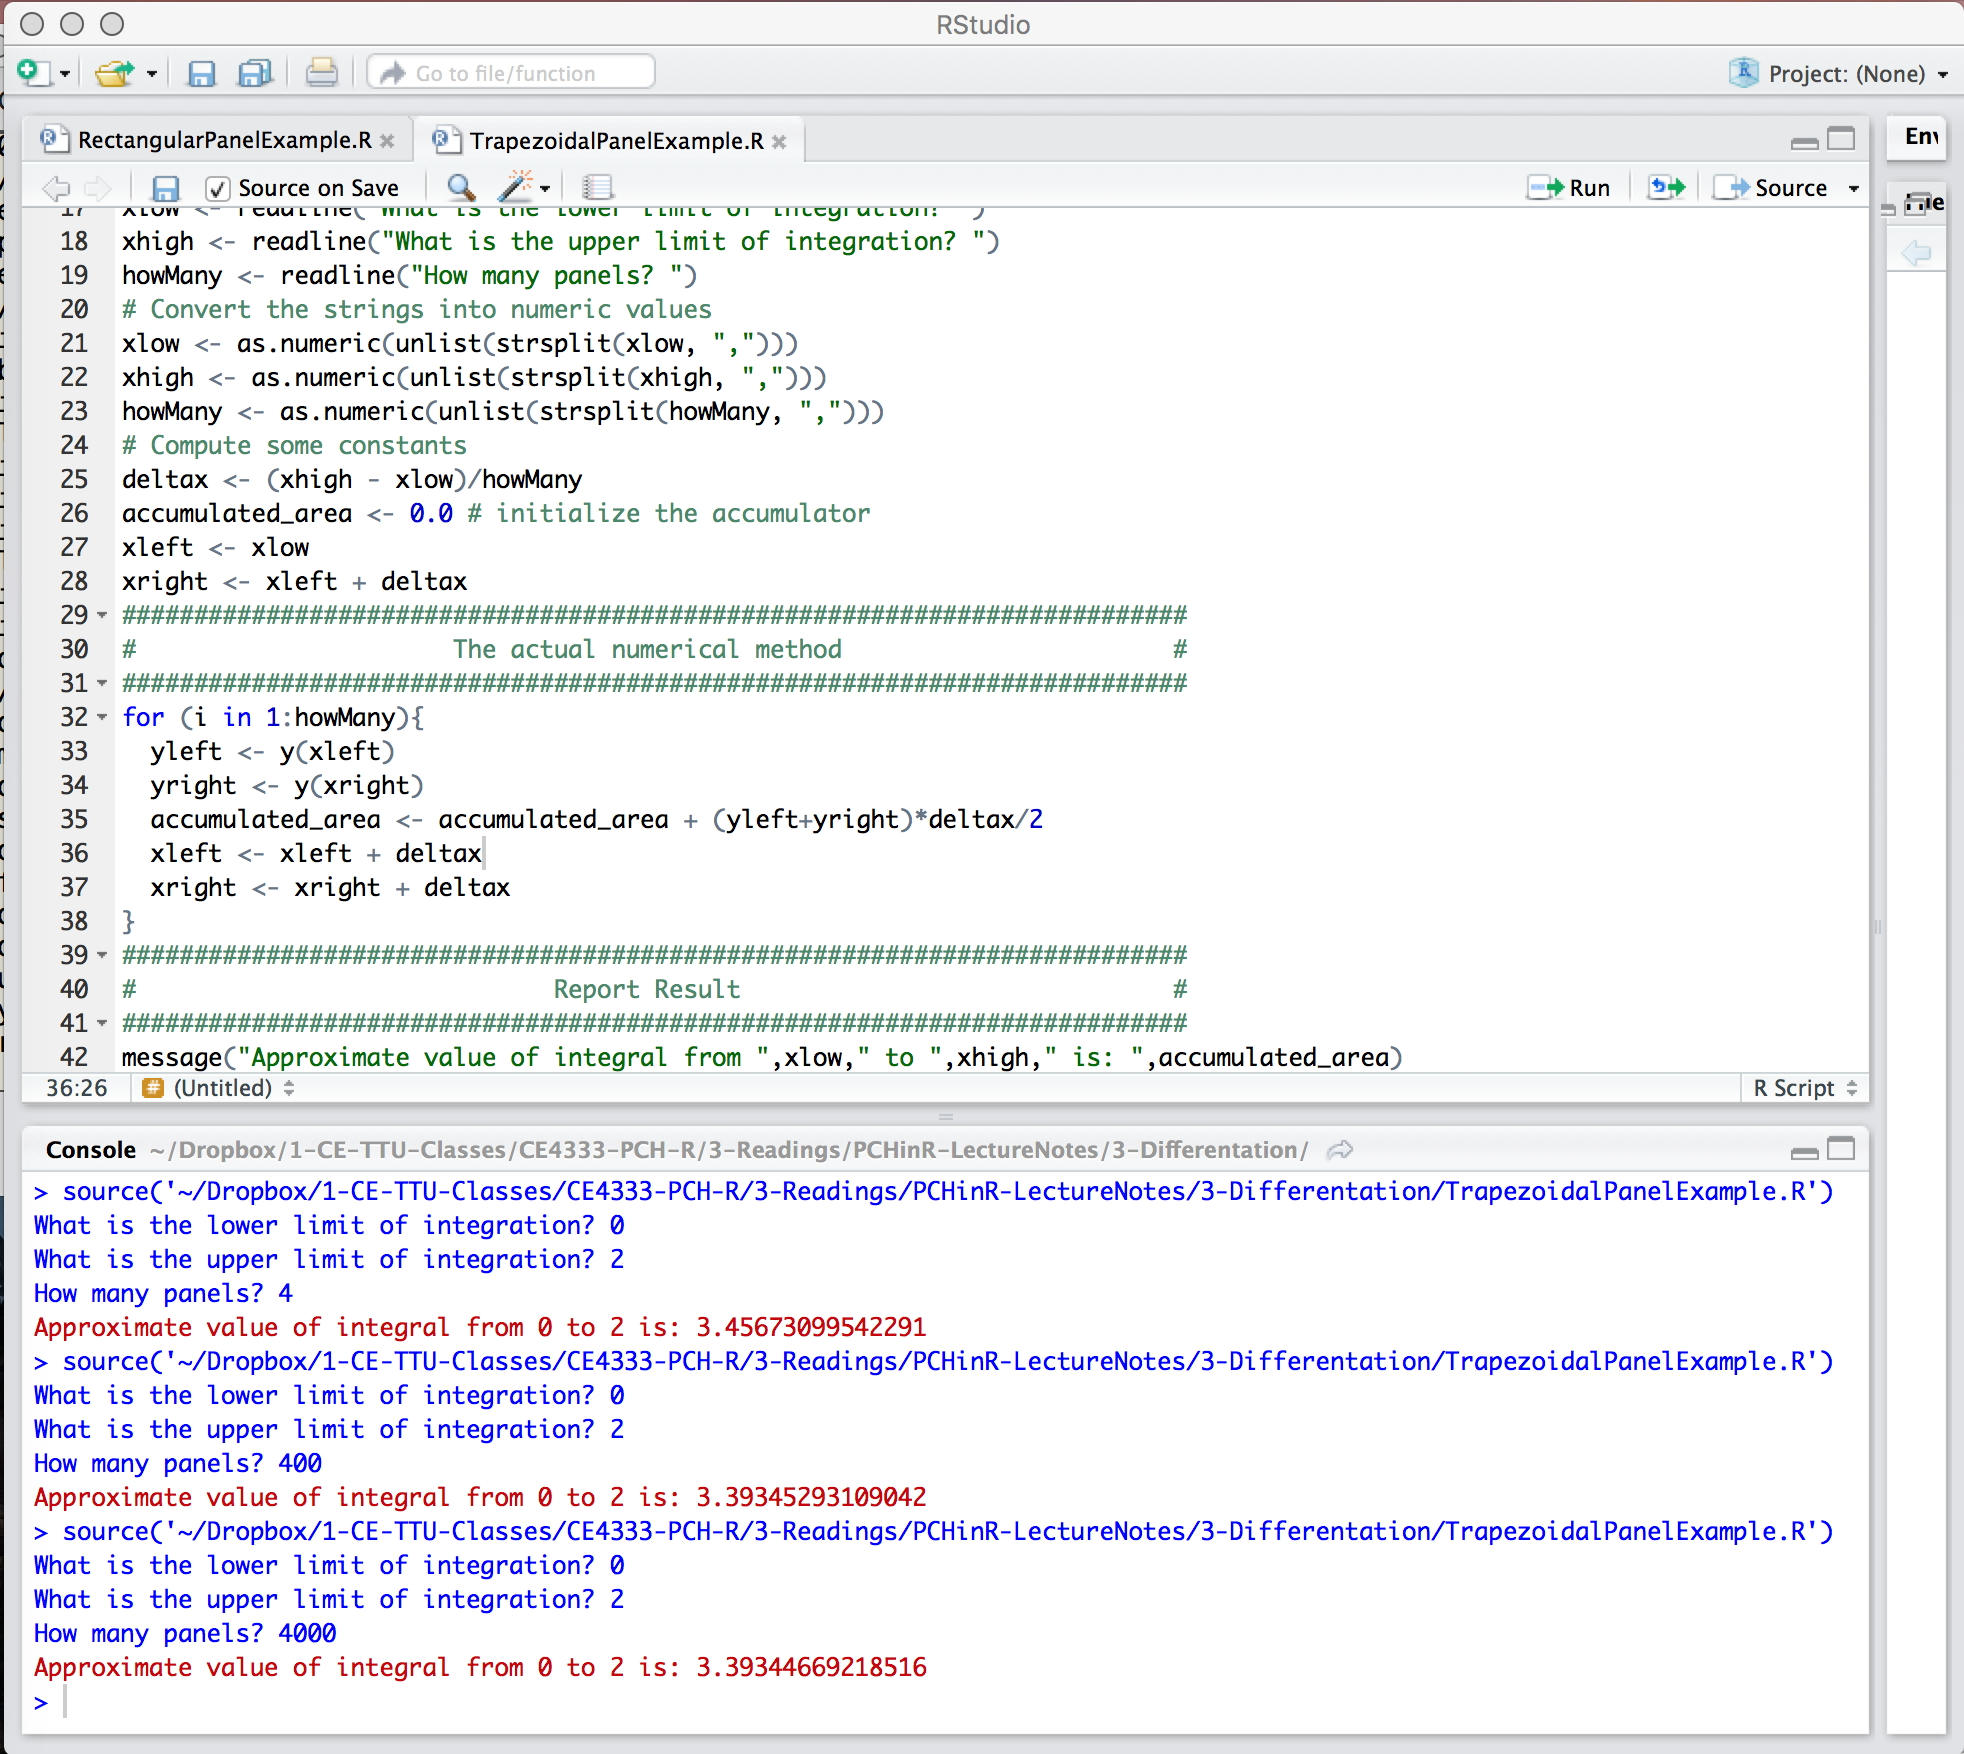
\includegraphics[width=6in]{./3-Differentation/TrapExample.jpg} 
   \caption{Trapezoidal panel example using 4, 400, and 4000 panels.}
   \label{fig:TrapExample}
\end{figure}

The actual listing depicted in Figure \ref{fig:TrapExample} is shown in Listing \ref{lst:TrapPanels}. 
Observe (at least for this example) the method appears more accurate that the rectangular method for the same number of panels, however also observe we are making twice as many function calls.
\clearpage

\begin{lstlisting}[caption=R code demonstrating Trapezoidal Panel Numerical Integration, label=lst:TrapPanels]
# R script to implement trapezoidal panel numerical integration
################################# NOTE ####################################
## The interactive input requires the script to be sourced                #
# In R console the command line would be                                  #
# source('PATH-TO-THE-FILE/TrapezoidalPanelExample.R')                    #
# where PATH-TO-THE-FILE is replaced with the actual path on your machine #
###########################################################################
#             Function to be integrated (modify as needed)                #
###########################################################################
y <- function(x){
  y <- x * sqrt(1+x^2)
  return(y)
}
###########################################################################
#             Get lower,upper and how many panels from user               #
###########################################################################
xlow <- readline("What is the lower limit of integration? ")  
xhigh <- readline("What is the upper limit of integration? ")
howMany <- readline("How many panels? ")
# Convert the strings into numeric values
xlow <- as.numeric(unlist(strsplit(xlow, ",")))
xhigh <- as.numeric(unlist(strsplit(xhigh, ",")))
howMany <- as.numeric(unlist(strsplit(howMany, ",")))
# Compute some constants
deltax <- (xhigh - xlow)/howMany  
accumulated_area <- 0.0 # initialize the accumulator
xleft <- xlow
xright <- xleft + deltax
##########################################################################
#                      The actual numerical method                       #
##########################################################################
for (i in 1:howMany){
  yleft <- y(xleft)
  yright <- y(xright)
  accumulated_area <- accumulated_area + (yleft+yright)*deltax/2
  xleft <- xleft + deltax
  xright <- xright + deltax
}
##########################################################################
#                             Report Result                              #
##########################################################################
message("Approximate value of integral from ",xlow," to ",xhigh," is: ",accumulated_area)
\end{lstlisting}

\subsubsection{Parabolic Panels}
Parabolic panels approximate the shape of the panel with a parabola.  The area between the chord and the curve (neglected in the trapezoidal solution) may be accounted for by approximating the function with a parabola passing through the points defined by three successive values of $y$.  

This area may be calculated from the geometry of the parabola and added to the trapezoidal area of the pair of strips to give the area $\Delta A$ of the pair as illustrated. Adding all of the $\Delta A$s produces the tabulation shown, which is known as Simpson's rule. To use Simpson's rule, the number $n$ of strips must be even.

\begin{figure}[h!] %  figure placement: here, top, bottom, or page
   \centering
   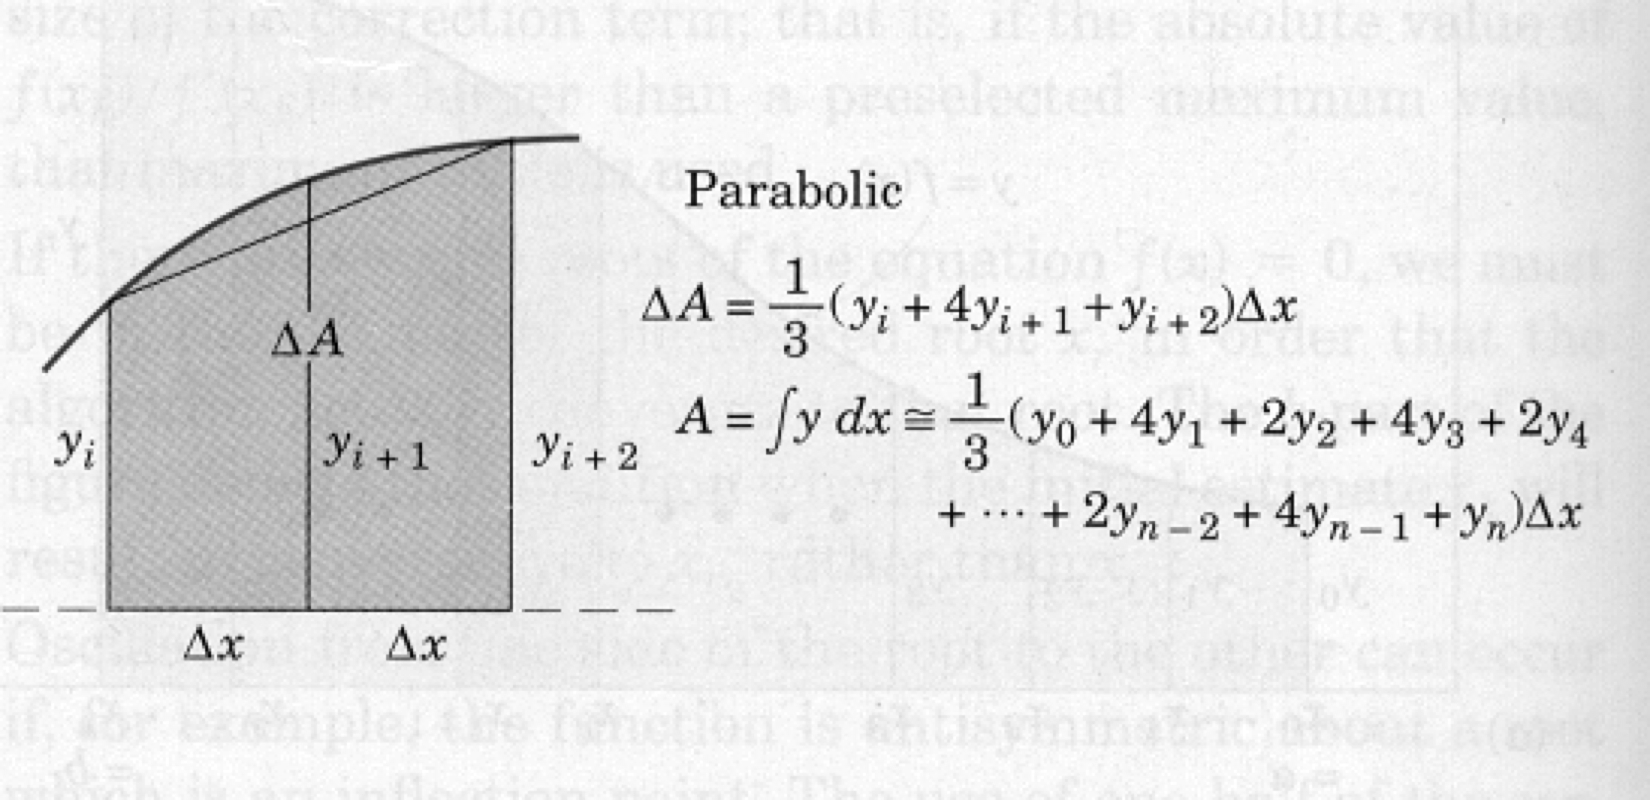
\includegraphics[width=5in]{./3-Differentation/ParabolicPanels.jpg} 
   \caption{Parabolic Panel Schematic.}
   \label{fig:ParabolicPanels}
\end{figure}

The same example as presented for rectangular panels is repeated, except using parabolic panels.  The code is changed yet again because we will evaluate at each end of the panel as well as at an intermediate value.

Figure \ref{fig:ParaExample} is a screen capture of a parabolic panel integration.   
The actual script is also listed in Listing \ref{lst:ParaPanels}. 
In the script, I substituted  $\frac{\Delta x}{2}$ for $\Delta x$ from Figure \ref{fig:ParabolicPanels}, so the accumulation line has a 6 in the denominator (rather than the 3 in the figure).\footnote{$\dots \frac{\Delta x}{2} \times \frac{1}{3}$ = $\dots \frac{\Delta x}{6}$}

\begin{figure}[h!] %  figure placement: here, top, bottom, or page
   \centering
   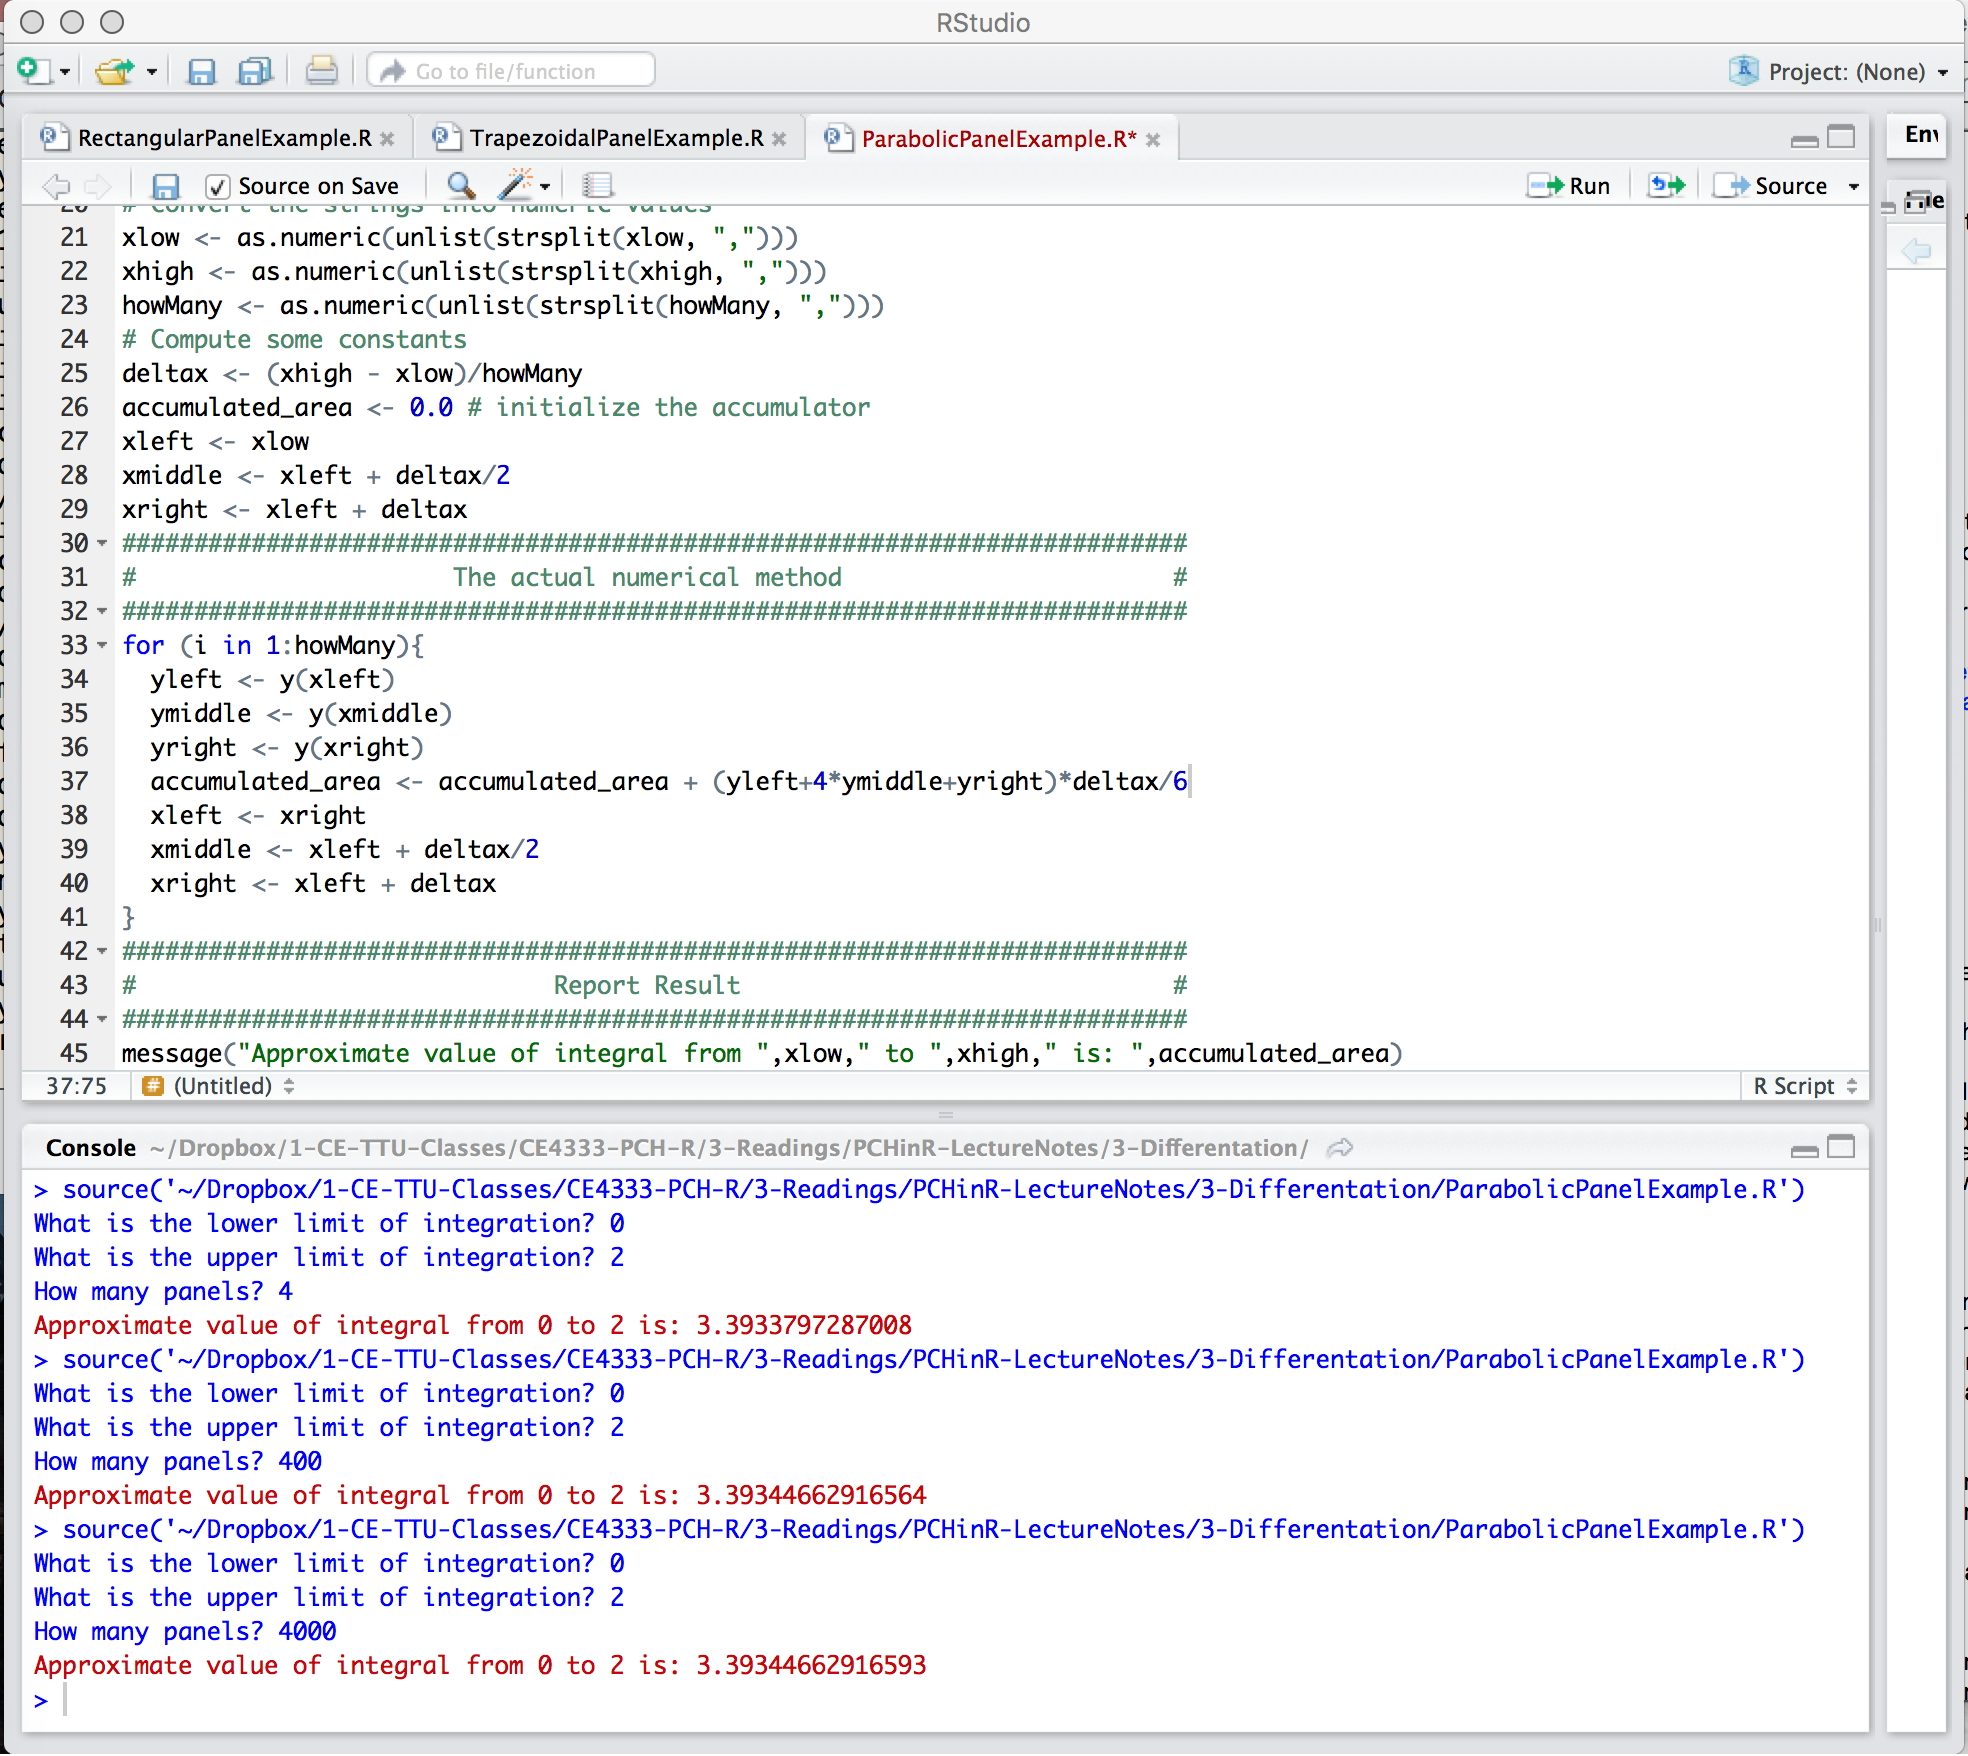
\includegraphics[width=6in]{./3-Differentation/ParaExample.jpg} 
   \caption{Parabolic panel example using 4, 400, and 4000 panels}
   \label{fig:ParaExample}
\end{figure}

Observe that the estimated integral for 400 and 4000 panels is nearly the same, suggesting no need to go beyond a certain number of panels.  
Algorithms that detect when to stop adding panels exist and would be implemented in many scientific and engineering programming applications.

\begin{lstlisting}[caption=R code demonstrating Parabolic Panel Numerical Integration, label=lst:ParaPanels]
# R script to implement trapezoidal panel numerical integration
################################# NOTE ####################################
## The interactive input requires the script to be sourced                #
# In R console the command line would be                                  #
# source('PATH-TO-THE-FILE/RectangularPanelExample.R')                    #
# where PATH-TO-THE-FILE is replaced with the actual path on your machine #
###########################################################################
#             Function to be integrated (modify as needed)                #
###########################################################################
y <- function(x){
  y <- x * sqrt(1+x^2)
  return(y)
}
###########################################################################
#             Get lower,upper and how many panels from user               #
###########################################################################
xlow <- readline("What is the lower limit of integration? ")  
xhigh <- readline("What is the upper limit of integration? ")
howMany <- readline("How many panels? ")
# Convert the strings into numeric values
xlow <- as.numeric(unlist(strsplit(xlow, ",")))
xhigh <- as.numeric(unlist(strsplit(xhigh, ",")))
howMany <- as.numeric(unlist(strsplit(howMany, ",")))
# Compute some constants
deltax <- (xhigh - xlow)/howMany  
accumulated_area <- 0.0 # initialize the accumulator
xleft <- xlow
xmiddle <- xleft + deltax/2
xright <- xleft + deltax
##########################################################################
#                      The actual numerical method                       #
##########################################################################
for (i in 1:howMany){
  yleft <- y(xleft)
  ymiddle <- y(xmiddle)
  yright <- y(xright)
  accumulated_area <- accumulated_area + (yleft+4*ymiddle+yright)*deltax/6
  xleft <- xright
  xmiddle <- xleft + deltax/2
  xright <- xleft + deltax
}
##########################################################################
#                             Report Result                              #
##########################################################################
message("Approximate value of integral from ",xlow," to ",xhigh," is: ",accumulated_area)
\end{lstlisting}

If we study all the forms of the numerical method we observe that the numerical integration method is really the sum of function values at specific locations in the interval of interest, with each value multiplied by a specific weight. 
In this development the weights were based on polynomials, but other method use different weighting functions.  
An extremely important method is called gaussian quadrature, which is outside the scope of the discussion herein  --- Gaussian quadrature routines are readily available within \textbf{R}.
The method is valuable because one can approximate convolution integrals quite effectively using quadrature routines, while the number of function evaluations for a polynomial based approximation could become hopeless.

When the function values are tabular, we are going to have to accept the rectangular (with adaptations) and trapezoidal as our best tool to approximate an integral because we don't have any really effective way to evaluate the function between the tabulated values --  if we were to use our interpolation routine from earlier, its really going to be a kind of trapezoidal rule anyway.

\clearpage
\subsection{Exercise Set 2}
\begin{enumerate}
\item Write a script to approximate $\int_{1.8}^{3.4}e^x dx$ using rectangular panels.  \\Run your script using 6 and 600 panels.  
\begin{enumerate}
\item What is the analytical solution (e.g. do the calculus!)?  
\item What is the percent error between the analytical solution and the approximation using 6 panels?
\item What is the percent error between the analytical solution and the approximation using 600 panels?
\end{enumerate}
\item Write a script to approximate $\int_{1.8}^{3.4}e^x dx$ using trapezoidal panels.   \\Run your script using 6 and 600 panels.  
\begin{enumerate}
\item What is the analytical solution (e.g. do the calculus!)?  
\item What is the percent error between the analytical solution and the approximation using 6 panels?
\item What is the percent error between the analytical solution and the approximation using 600 panels?
\end{enumerate}
\item Based on the previous two exercises, which method do you think is more accurate for a given panel count?  Why (do you think so)?
\item Write a script to approximate $\int_{0}^{1}ln(x) dx$ using rectangular panels.  \\Run your script using 6 and 600 panels.  
\begin{enumerate}
\item What is the analytical solution (e.g. do the calculus!)?  
\item What is the percent error between the analytical solution and the approximation using 6 panels?
\item What is the percent error between the analytical solution and the approximation using 600 panels?
\end{enumerate}

\item Write a script to approximate $\int_{0}^{1}ln(x) dx$ using trapezoidal panels.  \\Run your script using 6 and 600 panels.  
\begin{enumerate}
\item Did you get an error message --- why?
\end{enumerate}

\end{enumerate}

This exercise set is also located on the class server as \texttt{ES-2}
\clearpage

\subsection{Numerical Integration of Tabular Data}
This subsection is going to work with tabular data --- different from function evaluation, but similar.  
To be really useful, we need to learn how to read data from a file --- manually entering tabular data is really time consuming, error prone, and just plain idiotic.

So in this subsection we will first learn how to read data from a file into a list, then we can process the list as if it were a function and integrate its contents.   %I am probably going to dispense with cuteness for awhile --- file reads and writes are complex in any language, so you have to adult (as a verb) for a little while --- sorry!

\subsubsection{Reading from a file -- open, read, close files}
\textbf{R} can read from an ASCII file (or even an Excel .csv file) using a multitude of methods.  Common methods are \texttt{read.table(\dots )}, \texttt{read.table(\dots )}, \texttt{read.table(\dots )}, \texttt{read.table(\dots )}, and \texttt{read.table(\dots )}.

One can also use primatives\footnote{Jargon to describe lower level tools within \textbf{R}} to read individual rows in a file and process them.\footnote{We will use this approach later in the book -- the interactive prompt and reads in the prior subsection are similar to this approach where input is read into a string, then the string is converted into the appropriate type of object (numeric or text).}

First, lets create a file named \texttt{MyFile.txt}.
The extension is important so that we can examine the file with other tools (a text editor) and remember that it is an ASCII file.
The contents of \texttt{MyFile.txt} are:
\begin{verbatim}
1 , 1
2 , 4
3 , 9
4 , 16
5 , 25
\end{verbatim}

To read the contents into an \textbf{R} script we have to do the following:
\begin{enumerate}
\item Open a connection to the file --- this is a concept common to all languages, it might be called something different, but the program needs to somehow know the location and name of the file.
\item Read the contents into an object --- we have a lot of control on how this gets done, for the time being we won't exercise much control yet.  When you do substantial programs, you will depend on the control of the reads (and writes).
\item Disconnect the file --- this too is common to all languages.  Its a really easy step to forget.  Not a big deal if the program ends as planned but terrible if there is a error in the program and the connection is still open.  Usually noting bad happens, but with an open connection it is possible for the file to get damaged.   If that file represents millions of customers data, that's kind of a problem.
\end{enumerate}
\newpage
The \texttt{read.table} class of functions handles all three of these steps for us, we do have to provide the filename and some information about the file structure.  Later when we are doing network simulation and other hydraulic techniques, different parts of an input file will be read line-by-line and processed --- for this task we will need to handle these three steps using primatives.

Figure \ref{fig:ReadMyFile} illustrates the process.  The input file has 5 lines, these get read then echoed (printed) back to us.  The actual script is pretty simple, notice how the \texttt{filepath} and \texttt{filename} character variables are defined, then pasted together to produce a full \textit{absolute} file name.\footnote{A file name can specify all the directory names starting from the root of the tree; then it is called an absolute file name. Or it can specify the position of the file in the tree relative to a default directory; then it is called a relative file name. On the computer I used to write this workbook, the symbol \~ ~, is the root to my user account, then the remaining directories from that location are explicitly listed.  The actual absolute name is 
/Users/cleveland/Dropbox/1-CE-TTU-Classes/CE4333-PCH-R/3-Readings/PCHinR-LectureNotes/3-Differentation/RScripts}

Listing \ref{lst:ReadMyFile} is a listing of the script used in Figure \ref{fig:ReadMyFile}.  
The analyst should be able to deduce that the filenames could be read from user input using the prompting technique used in the earlier subsections, so if one is going to process a lot of similar files the explicit naming could be replaced with variable naming -- it would probably be a good idea to confine the files to a reasonably memorable path.

\begin{figure}[h!] %  figure placement: here, top, bottom, or page
   \centering
   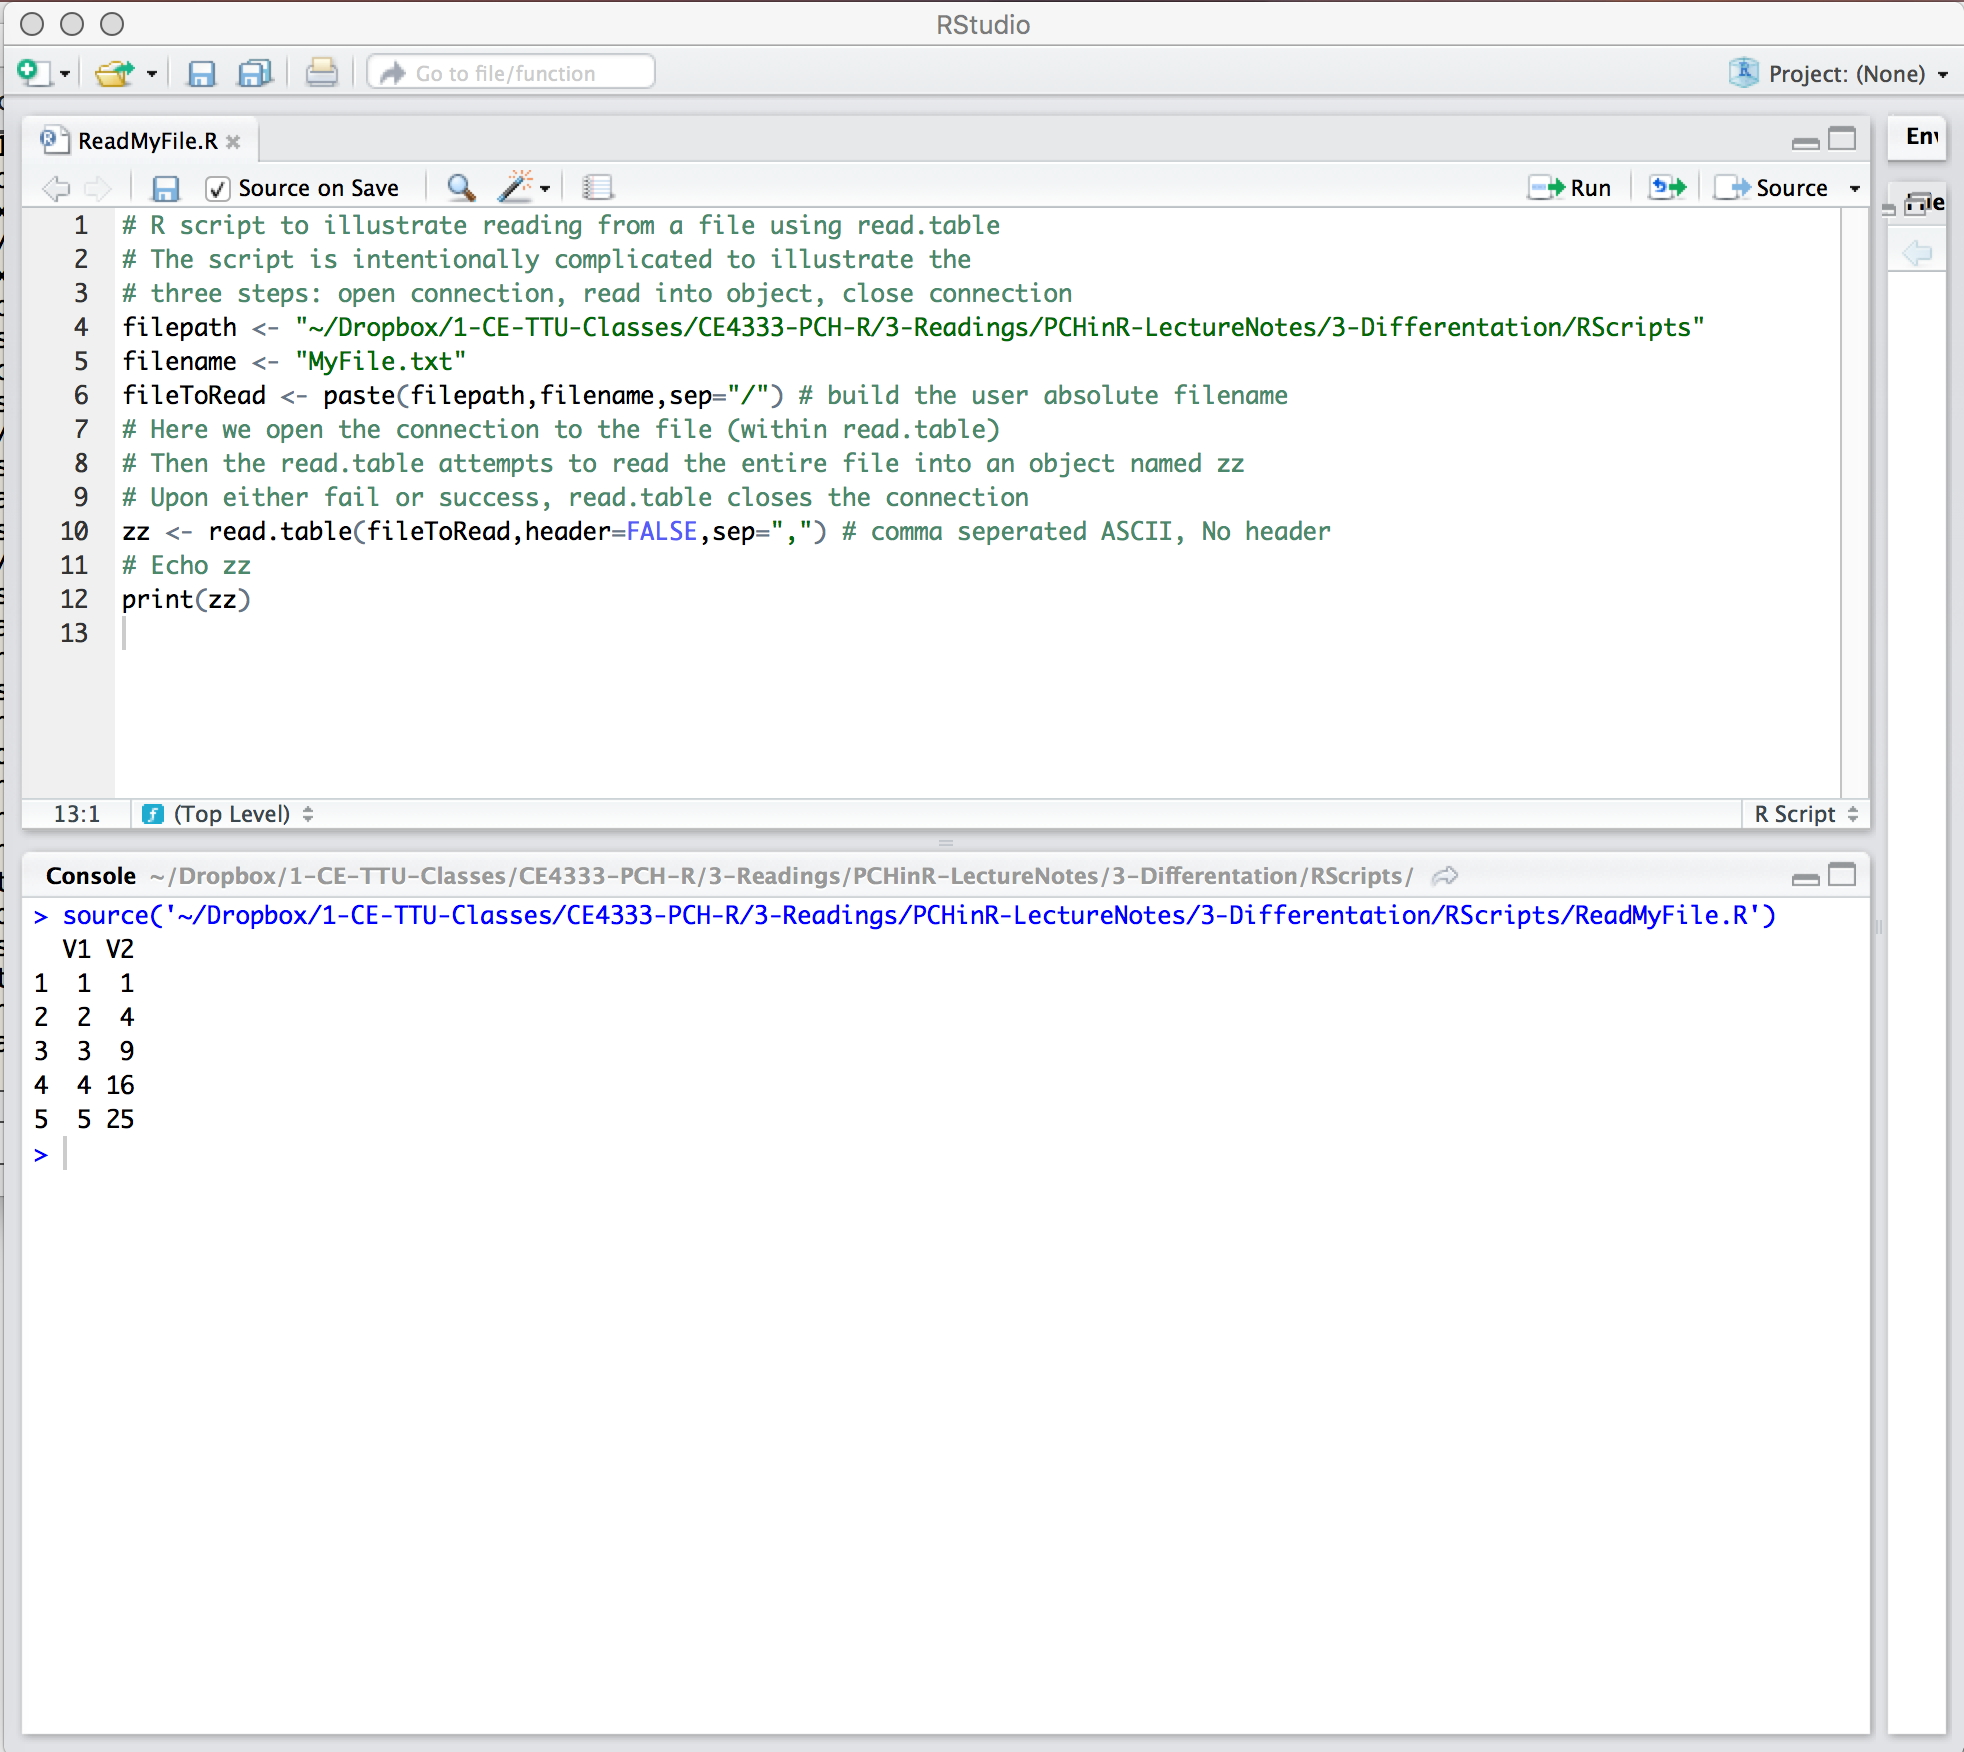
\includegraphics[width=6in]{./3-Differentation/ReadMyFile.jpg} 
   \caption{Rudimentary file reading}
   \label{fig:ReadMyFile}
\end{figure}

\begin{lstlisting}[caption=R code demonstrating Reading from a File, label=lst:ReadMyFile]
# R script to illustrate reading from a file using read.table
# The script is intentionally complicated to illustrate the 
# three steps: open connection, read into object, close connection
filepath <- "~/Dropbox/1-CE-TTU-Classes/CE4333-PCH-R/3-Readings/PCHinR-LectureNotes/3-Differentation/RScripts"
filename <- "MyFile.txt"
fileToRead <- paste(filepath,filename,sep="/") # build the user absolute filename
# Here we open the connection to the file (within read.table)
# Then the read.table attempts to read the entire file into an object named zz
# Upon either fail or success, read.table closes the connection
zz <- read.table(fileToRead,header=FALSE,sep=",") # comma seperated ASCII, No header
# Echo zz 
print(zz)
\end{lstlisting}

Now that we can read a file,  we are now able to integrate tabular data.

\subsection{Integrating tabular data}
Suppose instead of a function we only have tabulations and wish to estimate the area under the curve represented by the tabular values.  Then our integration rules from the prior sections still work more or less, except the rectangular panels will have to be shifted to either the left edge or right edge of a panel (where the tabulation exists).   

Lets just examine an example.  Suppose some measurement technology produced Table \ref{tab:MyIntegralTable} a table of related values.   The excitation variable is $x$ and $f(x)$ is the response.   

% Requires the booktabs if the memoir class is not being used
\begin{table}[h!]
   \centering
   \caption{Tabular values of an excitation--response relationship}
   \begin{tabular}{p{1in}p{1in}} 
   $x$ & $f(x)$ \\
   \hline
   \hline
   1.0 & 1.543 \\
   1.1 & 1.668 \\
   1.2 & 1.811 \\
   1.3 & 1.971 \\
   1.4 & 2.151 \\
   1.5 & 2.352 \\
   1.6 & 2.577 \\
   1.7 & 2.828 \\
   1.8 & 3.107 \\
   \hline
   \end{tabular}
   \label{tab:MyIntegralTable}
\end{table}

To integrate this table using the trapezoidal method is straightforward.  We will modify our earlier code to read the table (which we put into a file), and compute the integral.  

Figure \ref{fig:MyTrapTab} is a screen capture of a script that implements the file read and the numerical integration.
The conversion of the method from the functional form in the previous section is pretty straightforward.  
The main nusiance here is the syntax required to access the ``x'' values and the ``y'' values.   
In \textbf{R} the most generic approach is \texttt{object\$name}, where \textit{object} is the data frame name, and \textit{name} is the variable (column) name.  If you don't use headers, \textbf{R} assigns names as \texttt{V1,V2,\dots,V$_{max}$}.   

\begin{figure}[h!] %  figure placement: here, top, bottom, or page
   \centering
   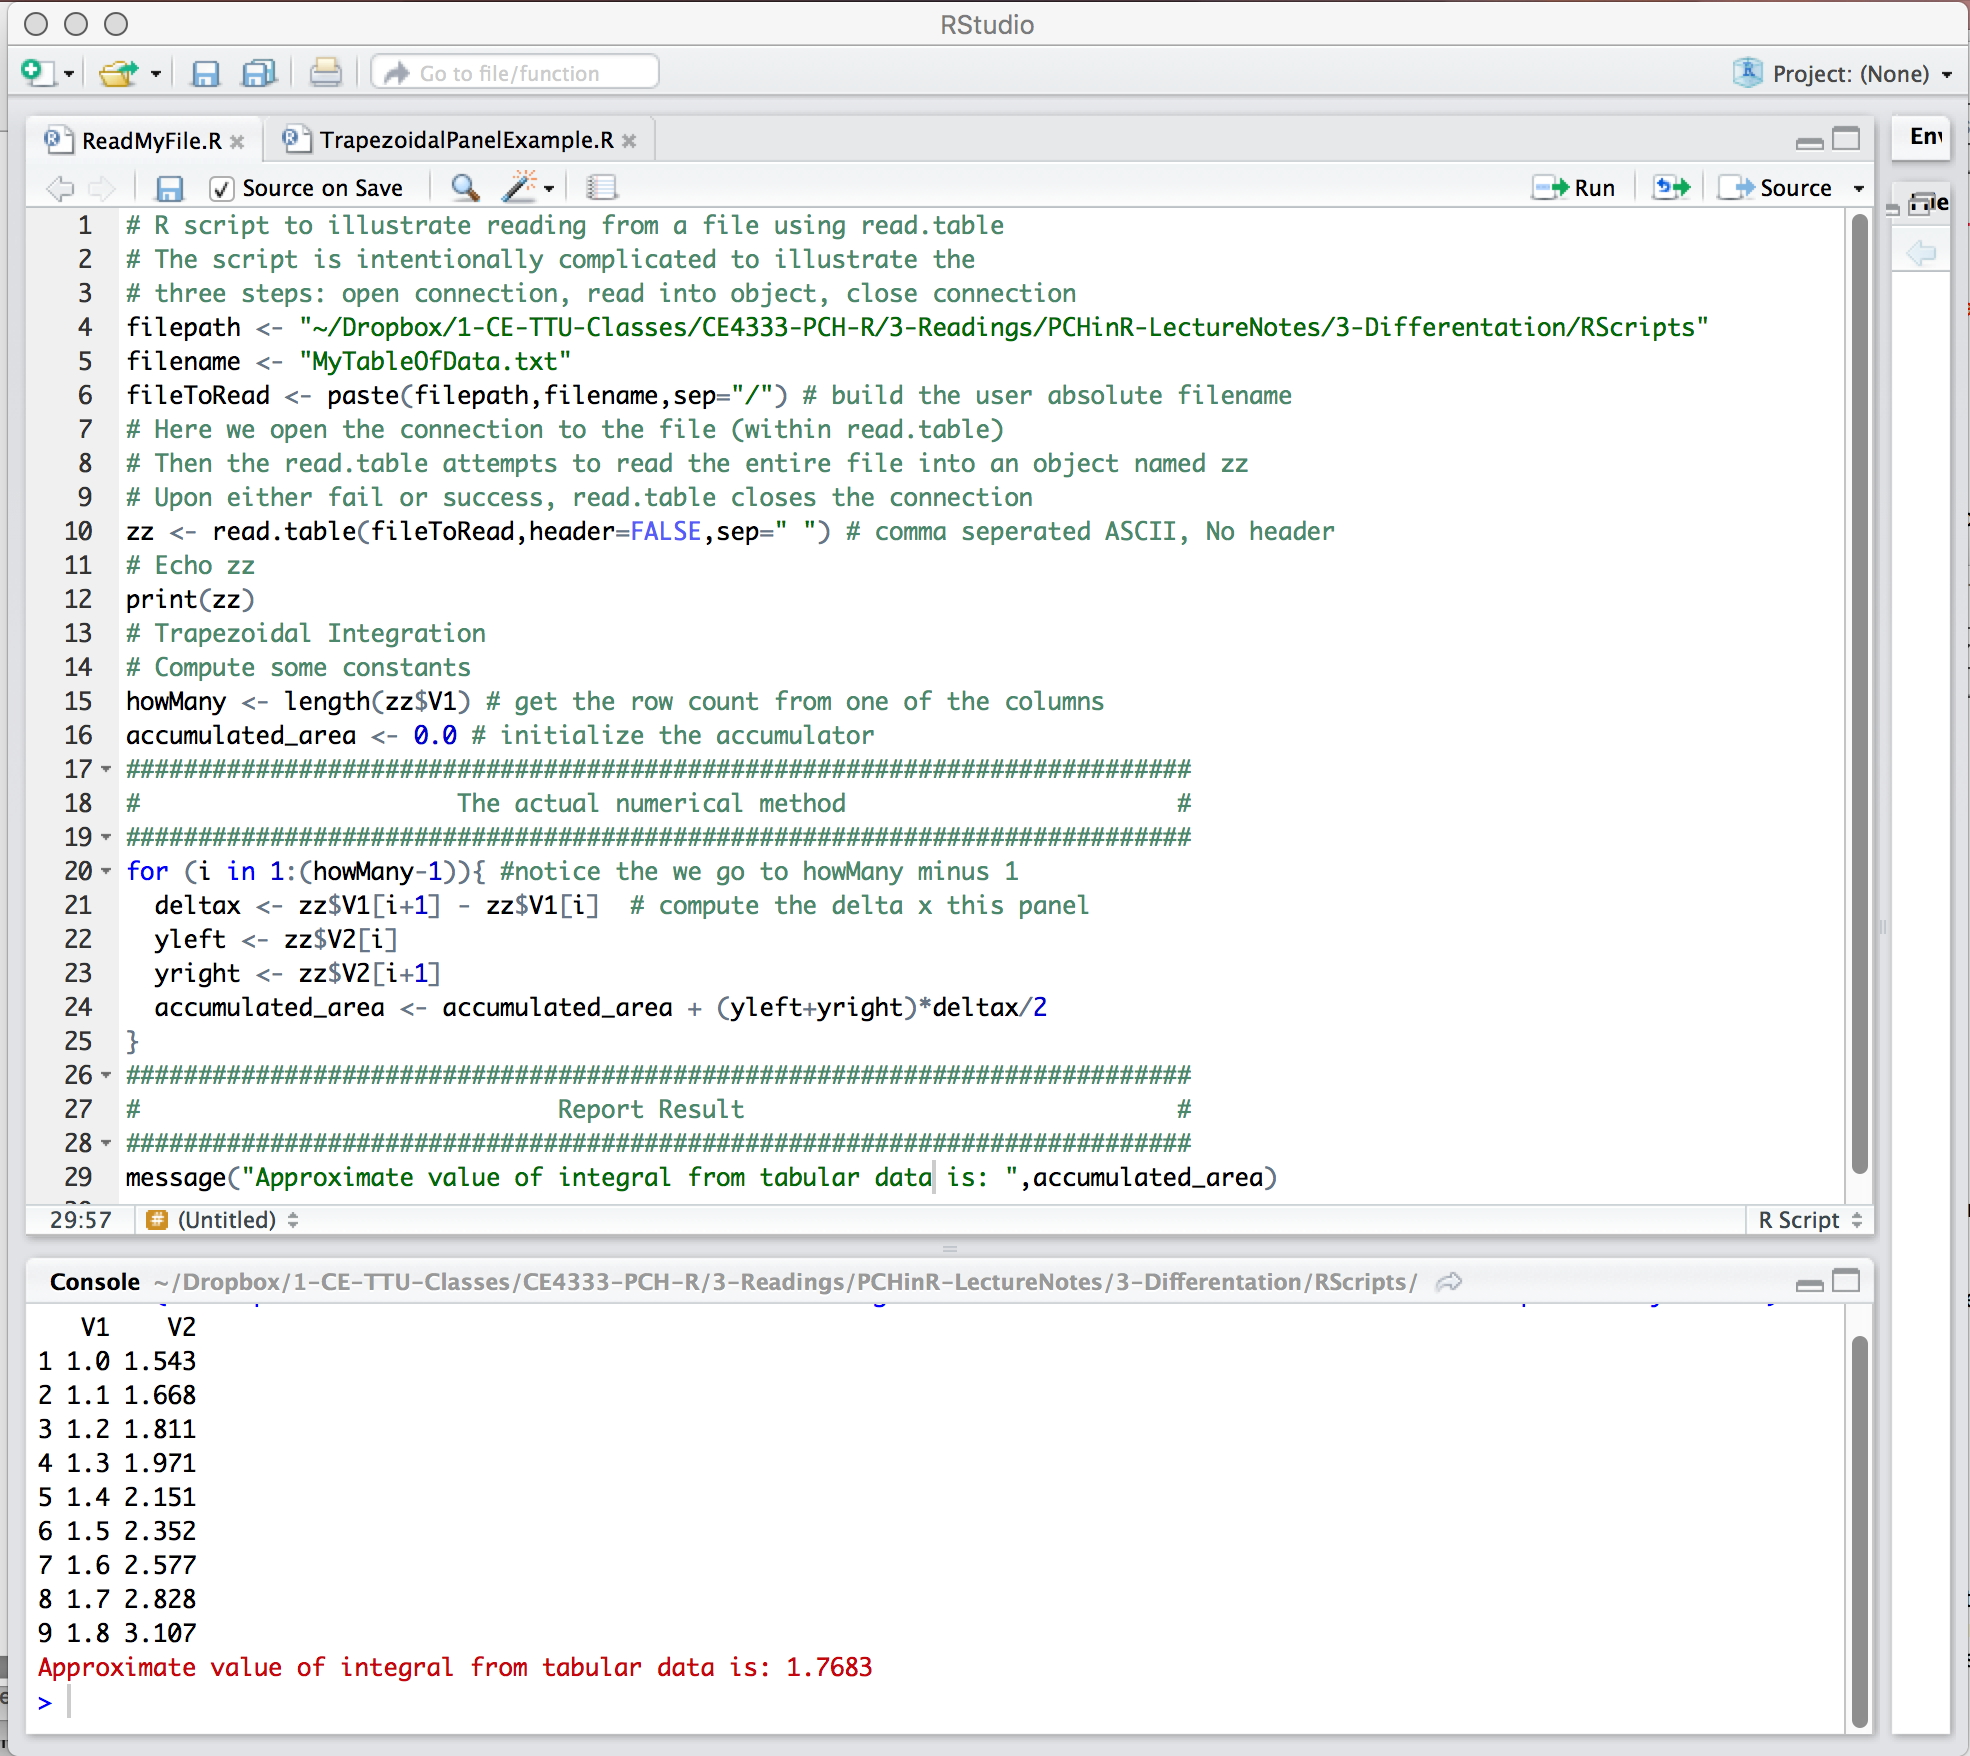
\includegraphics[width=6in]{./3-Differentation/MyTrapTab.jpg} 
   \caption{Integrating tabular data.}
   \label{fig:MyTrapTab}
\end{figure}

Realistically the only other simple integration method for tabular data is the rectangular rule, either using the left edge of a panel or the right edge of a panel (and you could do both and average the result which would result in the same outcome as the trapezoidal method).   For the sake of completeness lets do both and then compare the results from all four approaches (trapezoidal, rectangular-left, rectangular-right, average rectangular).

First, Figure \ref{fig:MyRectLeft} implements the file read and tabular integration using the rectangular panel method, evaluating the function at the left edge of each panel.

\begin{figure}[h!] %  figure placement: here, top, bottom, or page
   \centering
   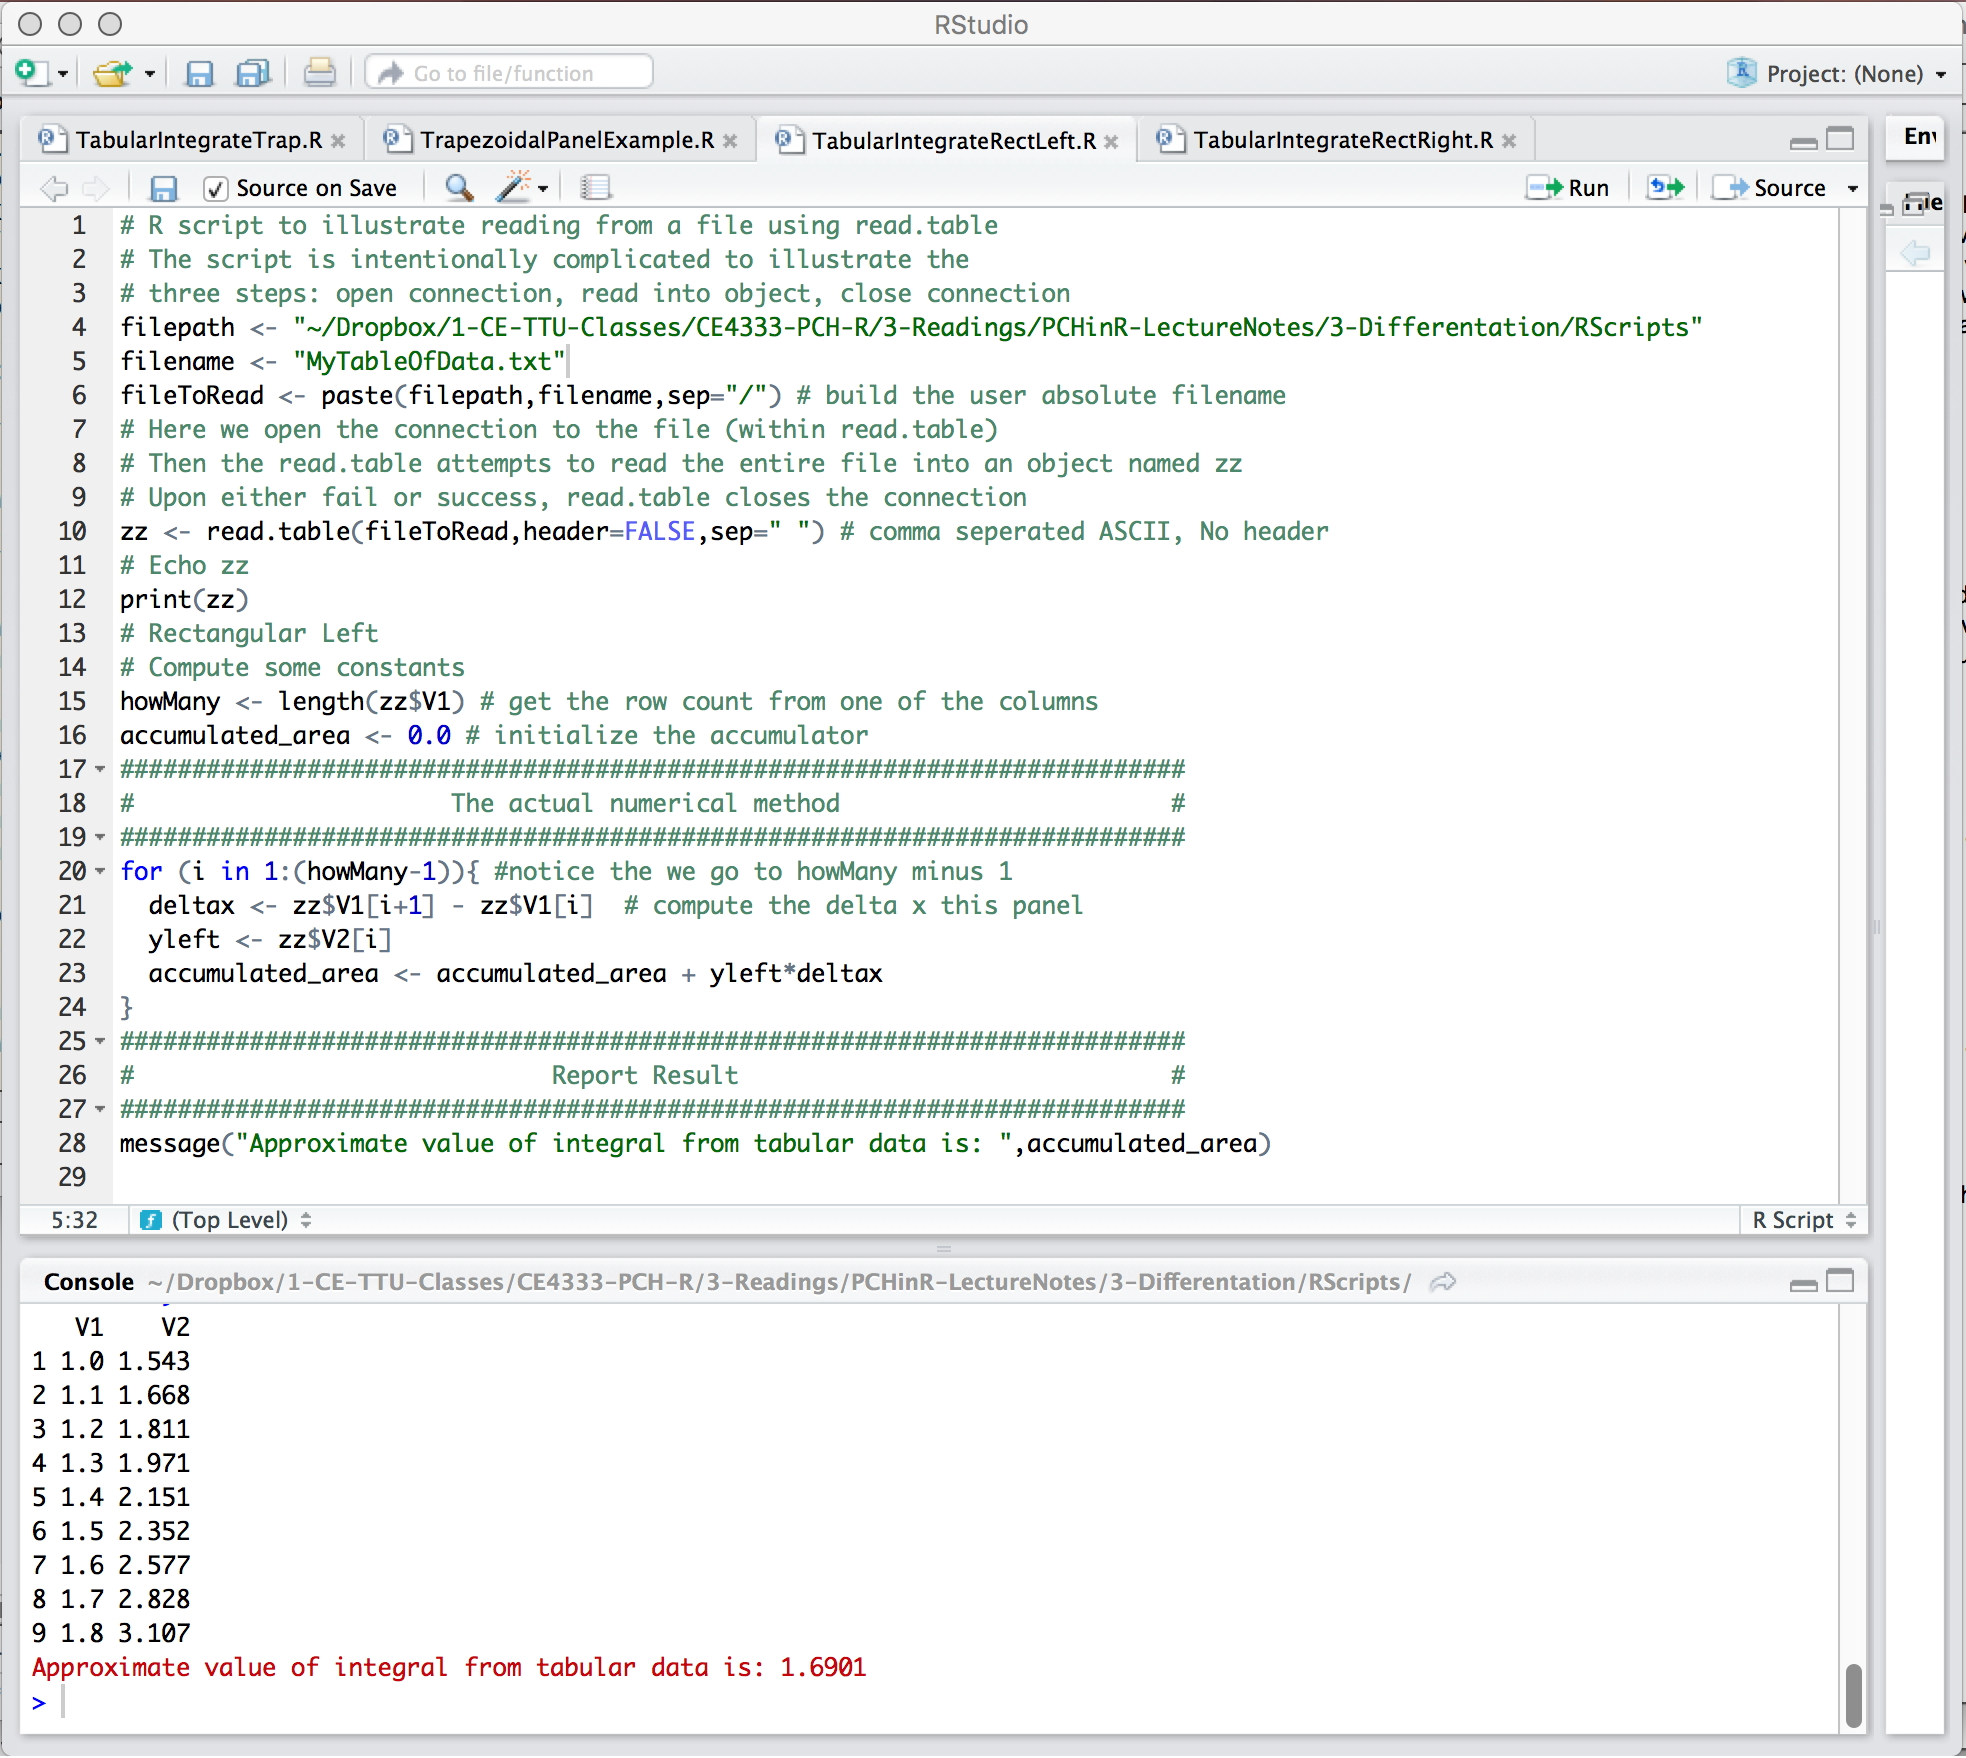
\includegraphics[width=6in]{./3-Differentation/MyRectLeft.jpg} 
   \caption{Integrating tabular data.   Rectangular panel, evaluate at left edge.}
   \label{fig:MyRectLeft}
\end{figure}

Next, Figure \ref{fig:MyRectRight} implements the file read and tabular integration using the rectangular panel method, evaluating the function at the left edge of each panel.

Now lets compare the results from using the three (four) approaches.  Table \ref{tab:MyTabularMethodCompare} are the results by method.   
% Requires the booktabs if the memoir class is not being used
\begin{table}[h!]
   \centering
   \caption{Comparison of tabular integration}
   \begin{tabular}{p{2.5in}p{2in}} 
   Method & Computed Area \\
   \hline
   \hline
Trapezoidal Panels & 1.7683 \\
Rectangular - Left Edge & 1.6901 \\
Rectangular - Right Edge & 1.8465 \\
Arithmetic Mean Rectangular & 1.7683  \\
   \hline
   \end{tabular}
   \label{tab:MyTabularMethodCompare}
\end{table}

What Table \ref{tab:MyTabularMethodCompare} illustrates is that the trapezoidal rule is simply the average of the rectangular rule evaluated at first the left-edge then the right-edge of a panel.   

\begin{figure}[t!] %  figure placement: here, top, bottom, or page
   \centering
   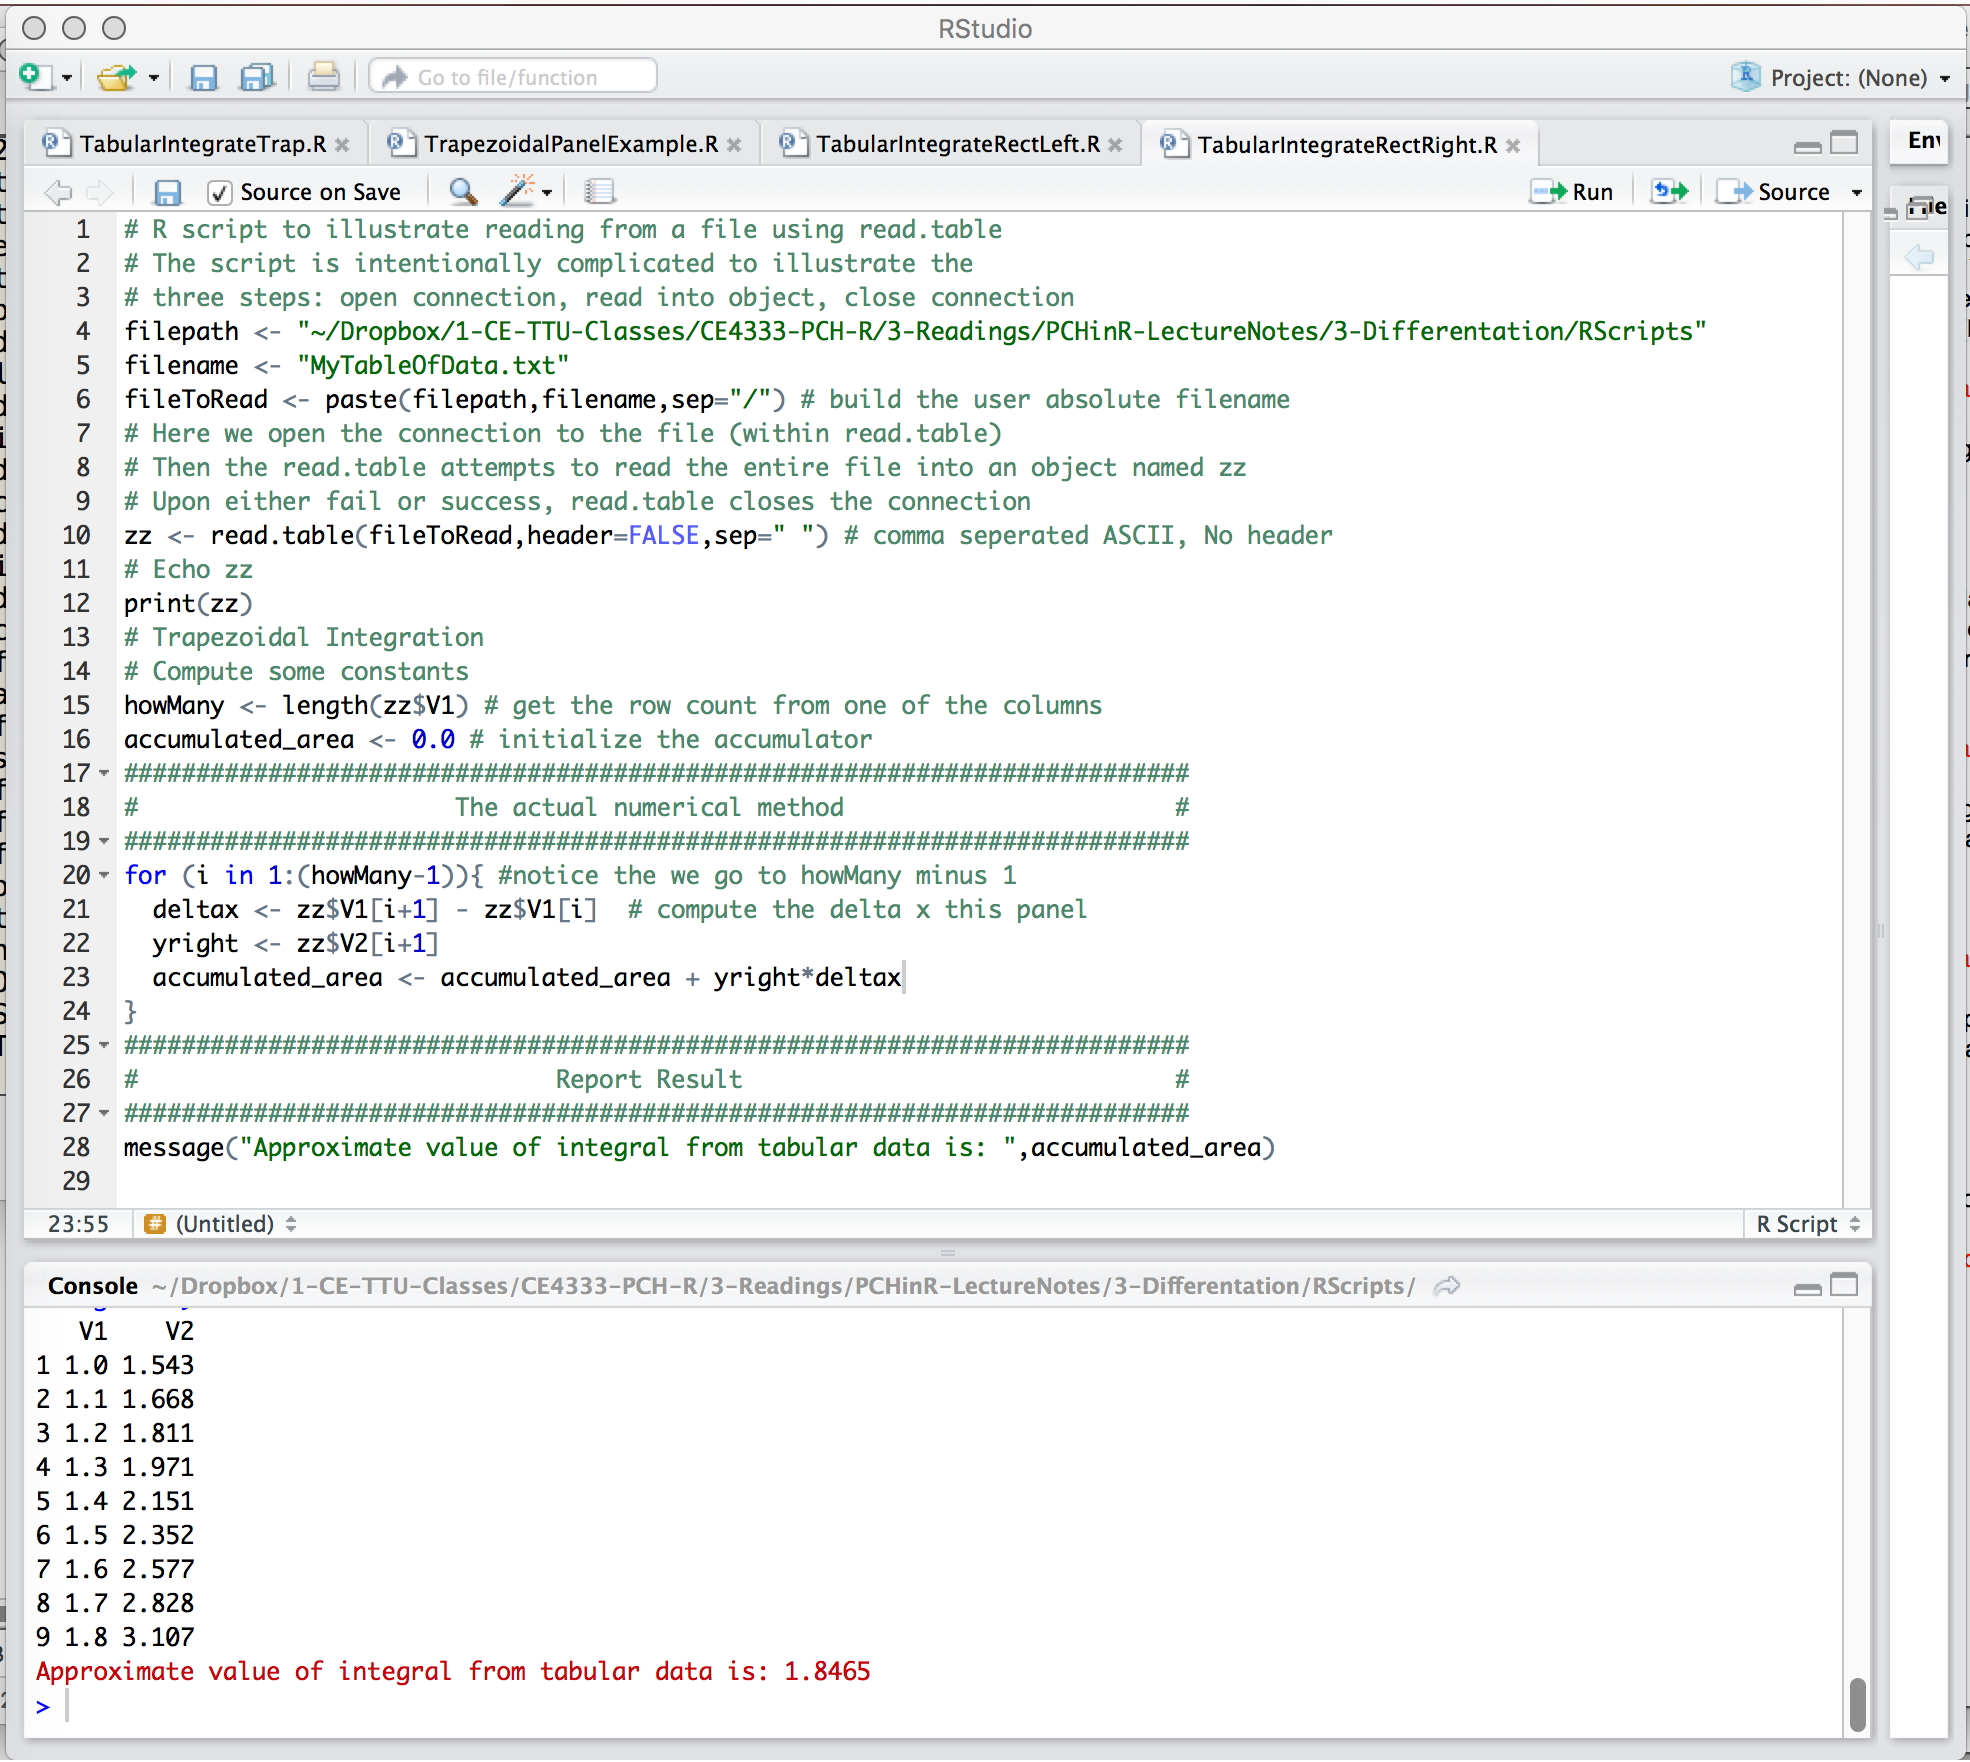
\includegraphics[width=6in]{./3-Differentation/MyRectRight.jpg} 
   \caption{Integrating tabular data.   Rectangular panel, evaluate at right edge.}
   \label{fig:MyRectRight}
\end{figure}

%\subsection{Exercises}
%\begin{enumerate}
%\item Approximate $\int_0^2 f(x) dx$ from the tabulation in Table \ref{tab:IntegrateThisProblem}.
%% Requires the booktabs if the memoir class is not being used
%\begin{table}[h!]
%   \centering
%   \caption{Tabular values of a function -- non-uniform spacing in $x$}
%   \begin{tabular}{p{1in}p{1in}} 
%   $x$ & $f(x)$ \\
%   \hline
%   \hline
%   0.00 & 1.0000 \\
%   0.12 & 0.8869 \\
%   0.53 & 0.5886 \\
%   0.87 & 0.4190 \\
%   1.08 & 0.3396 \\
%   1.43 & 0.2393 \\
%   2.00 & 0.1353 \\
%   \hline
%   \end{tabular}
%   \label{tab:IntegrateThisProblem}
%\end{table}
%\newpage
%\item Table \ref{tab:HyperbolicCosine} is a tabulation of various values of the hyperbolic cosine function.   
%\begin{enumerate}
%\item Approximate $\int_1^{9.0} f(x) dx$ from the tabulation in Table \ref{tab:HyperbolicCosine}.
%\item Approximate $\int_1^{4.2} f(x) dx$ from the tabulation in Table \ref{tab:HyperbolicCosine}.
%\item Approximate $\int_1^{4.0} f(x) dx$ from the tabulation in Table \ref{tab:HyperbolicCosine}.
%\item Briefly explain how you choose to handle starting and stopping the integration from values that are intermediate and within the tabulation.
%\item Also explain how you choose to handle  working with values that fall between tabulated values.
%\end{enumerate}
%\begin{table}[h!]
%   \centering
%   \caption{Tabular values of the hyperbolic cosine}
%   \begin{tabular}{p{1in}p{1in}} 
%   $x$ & $f(x)$ \\
%   \hline
%   \hline
%1.0 & 1.54308063481524 \\
%1.1 & 1.66851855382226 \\
%1.2 & 1.81065556732437 \\
%1.3 & 1.97091423032663 \\
%1.4 & 2.15089846539314 \\
%1.5 & 2.35240961524325 \\
%1.6 & 2.57746447119489 \\
%1.7 & 2.82831545788997 \\
%1.8 & 3.10747317631727 \\
%2.0 & 3.76219569108363 \\
%2.2 & 4.56790832889823 \\
%2.4 & 5.55694716696551 \\
%2.6 & 6.76900580660801 \\
%2.8 & 8.25272841686113 \\
%3.0 & 10.0676619957778 \\
%3.3 & 13.5747610440296 \\
%3.6 & 18.3127790830626 \\
%3.9 & 24.711345508488 \\
%4.2 & 33.3506633088728 \\
%4.6 & 49.7471837388392 \\
%5.0 & 74.2099485247878 \\
%5.5 & 122.348009517829 \\
%6.0 & 201.715636122456 \\
%7.0 & 548.317035155212 \\
%8.0 & 1490.47916125218 \\
%9.0 & 4051.54202549259 \\
%   \hline
%   \end{tabular}
%   \label{tab:HyperbolicCosine}
%\end{table}
%\end{enumerate}
%%%%%%%%%%%%%%%%%%%%%%%%%%%%%%%%%%%%%%%%%%%%%%%%%%%%%%%%
%%%%%%%%%%%%%%%%%%%%%%%%%%%%%%%%%%%%%%%%%%%%%%%%%%%%%%%%
\subsection{Numerical Differentiation}
Similar in context to numerical integration is approximation of derivatives.   
If the functions are representable as functions, then differencing degenerates into the selection of an appropriate difference formula.
If the function is tabular, the same decision is presented, but we have to pay additional attention to the quantity of observations available.

\subsection{Difference Approximations for Tabulated Data}
Here we will introduce differencing by an example.
Suppose we want to convert a cumulative data series into an incremental data series.  
It is operationally related to numerical differentiation.   

As an example (leading to an algorithm) consider the cumulative rainfall time series in Table \ref{tab:cumulative_rainfall_timeseries}.

We shall import this data into \textbf{R}, then plot the data, then construct a computational procedure to extract the incremental values from the cumulative values.
To load the data into \textbf{R} we start the program and then read the contents of a data file that contains the data into \textbf{R}, then we will introduce the plotting tools in \textbf{R}.
In addition to plotting, we will also learn about headers and attaching an object (which gives access to header names rather than the \texttt{object\$name} structure.

% Requires the booktabs if the memoir class is not being used
\begin{table}[ht!]
\centering
\caption{Cumulative Rainfall Time Series}
\begin{tabular}{cc} % Column formatting, @{} suppresses leading/trailing space
~&~\\
  hours & cumulative\_rain\\
  0.0&0.00\\
  0.5&1.06\\
  1.0&2.99\\
 1.5&4.80\\
 2.0&4.80\\
 2.5&4.80\\
 3.0&4.80\\
 3.5&4.80\\
 4.0&4.80\\
 4.5&4.80\\
 5.0&4.80\\
 5.5&4.80\\
\end{tabular}
\label{tab:cumulative_rainfall_timeseries}
\end{table}


\begin{figure}[htbp] %  figure placement: here, top, bottom, or page
   \centering
   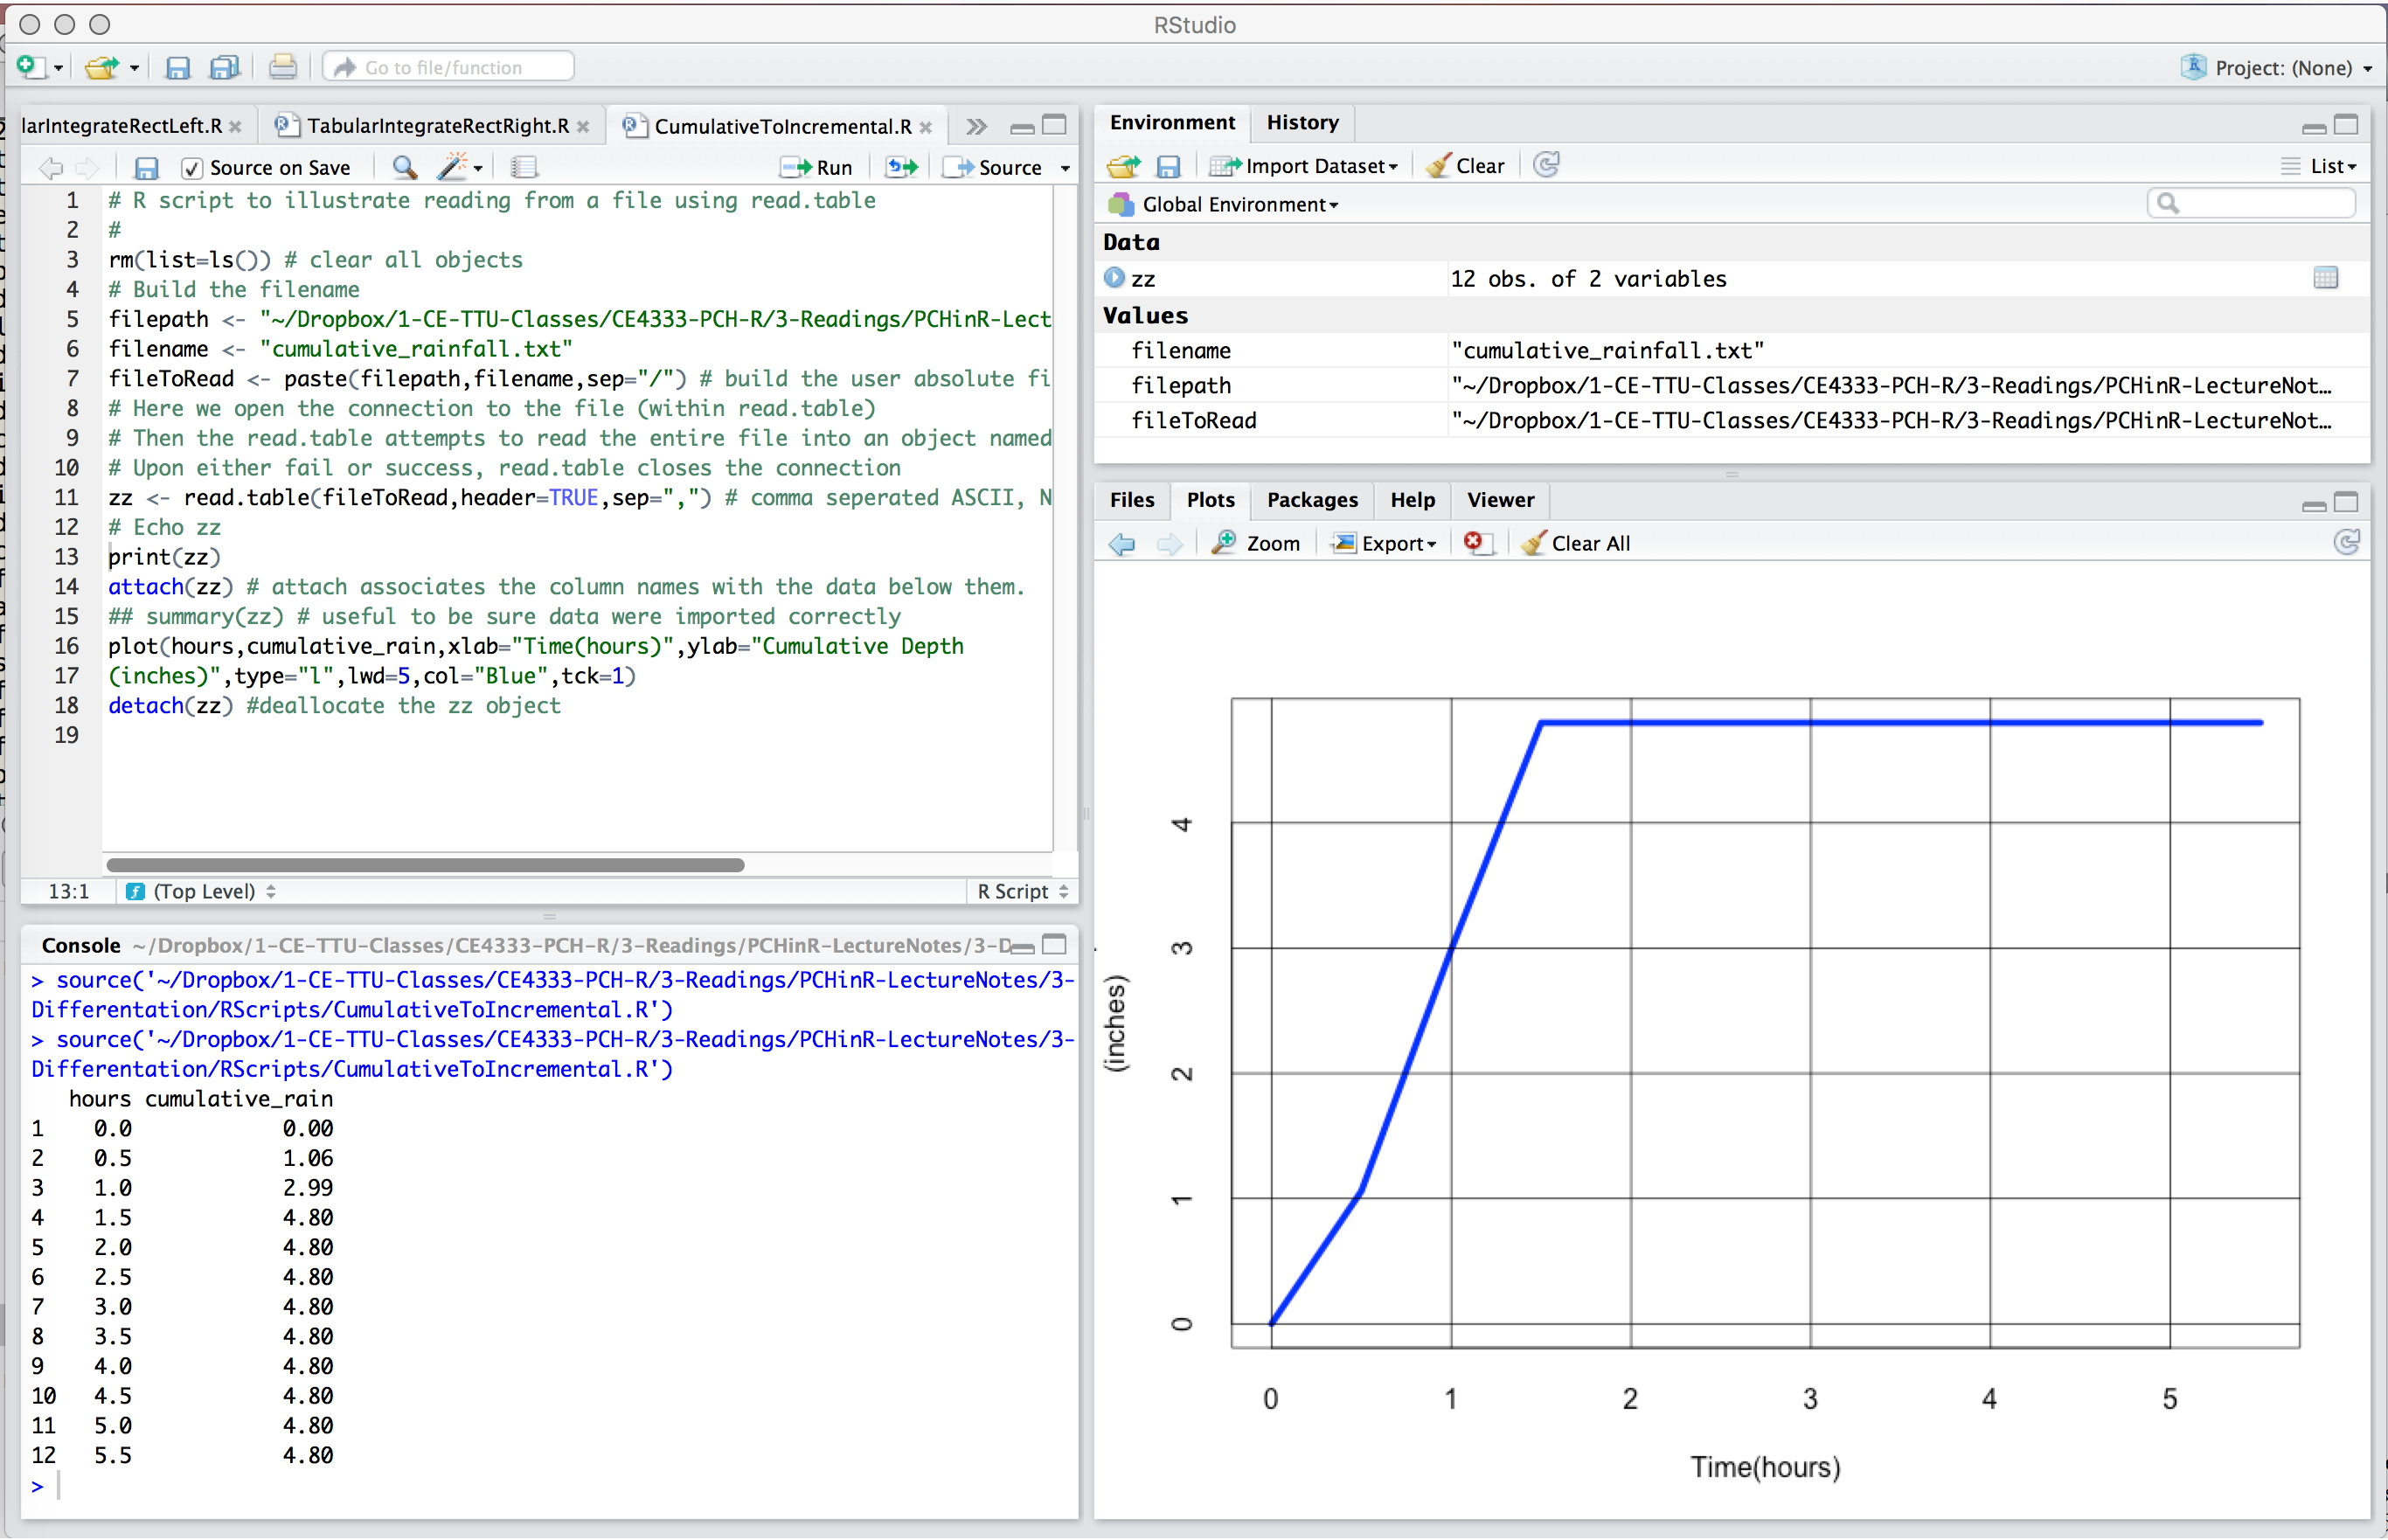
\includegraphics[width=6in]{./3-Differentation/cumulative_rain_plot.jpg} 
   \caption{Plot of Cumulative Rainfall Time Series}
   \label{fig:cumulative_rain_plot}
\end{figure}

The plot suggests that the values are accumulated at the end of the time interval, thus the value accumulated is some average ``rate'' multiplied by the time interval.  
The line segment between each point is called a ``secant'' line.  
The slope of each secant line, provides that average ``rate''.  
So a fundamental computational step will be a function that computes the slope given any two points (assumed to be adjacent --- so that's why sorting can become important, although the program doesn't actually care).

\subsubsection{Slope of a Secant Line}
\texttt{slopeOfSecant} is a prototype function that we write to that computes the slope of the secant line through two known points on a function $f(x_1)$ and $f(x_2)$.  The function could be tabular or evaluated.  The script assumes tabular in that the function is evaluates external to \texttt{slopeOfSecant}.  

\begin{lstlisting}[caption=R code demonstrating the prototype function \texttt{slopeOfSecant} , label=lst:SlopeOfSecant]
############## slope function prototype ####################
slopeOfSecant<-function(f1,f2,x1,x2){
  slopeOfSecant <- (f2-f1)/(x2-x1);
  return(slopeOfSecant)
}
#######################################################
\end{lstlisting}

This slope is also a first order approximation of a derivative (forward, backward, and centered differences depending on values supplied).  This function can then be used to compute ``derivatives'' of data series using a disaggregation function.

As an illustrative example, if we present parts of the cumulative rainfall data series we can recover the average rate between the inputs.  Figure \ref{fig:addSecant} is a screen capture of such a test.

\begin{figure}[htbp] %  figure placement: here, top, bottom, or page
   \centering
   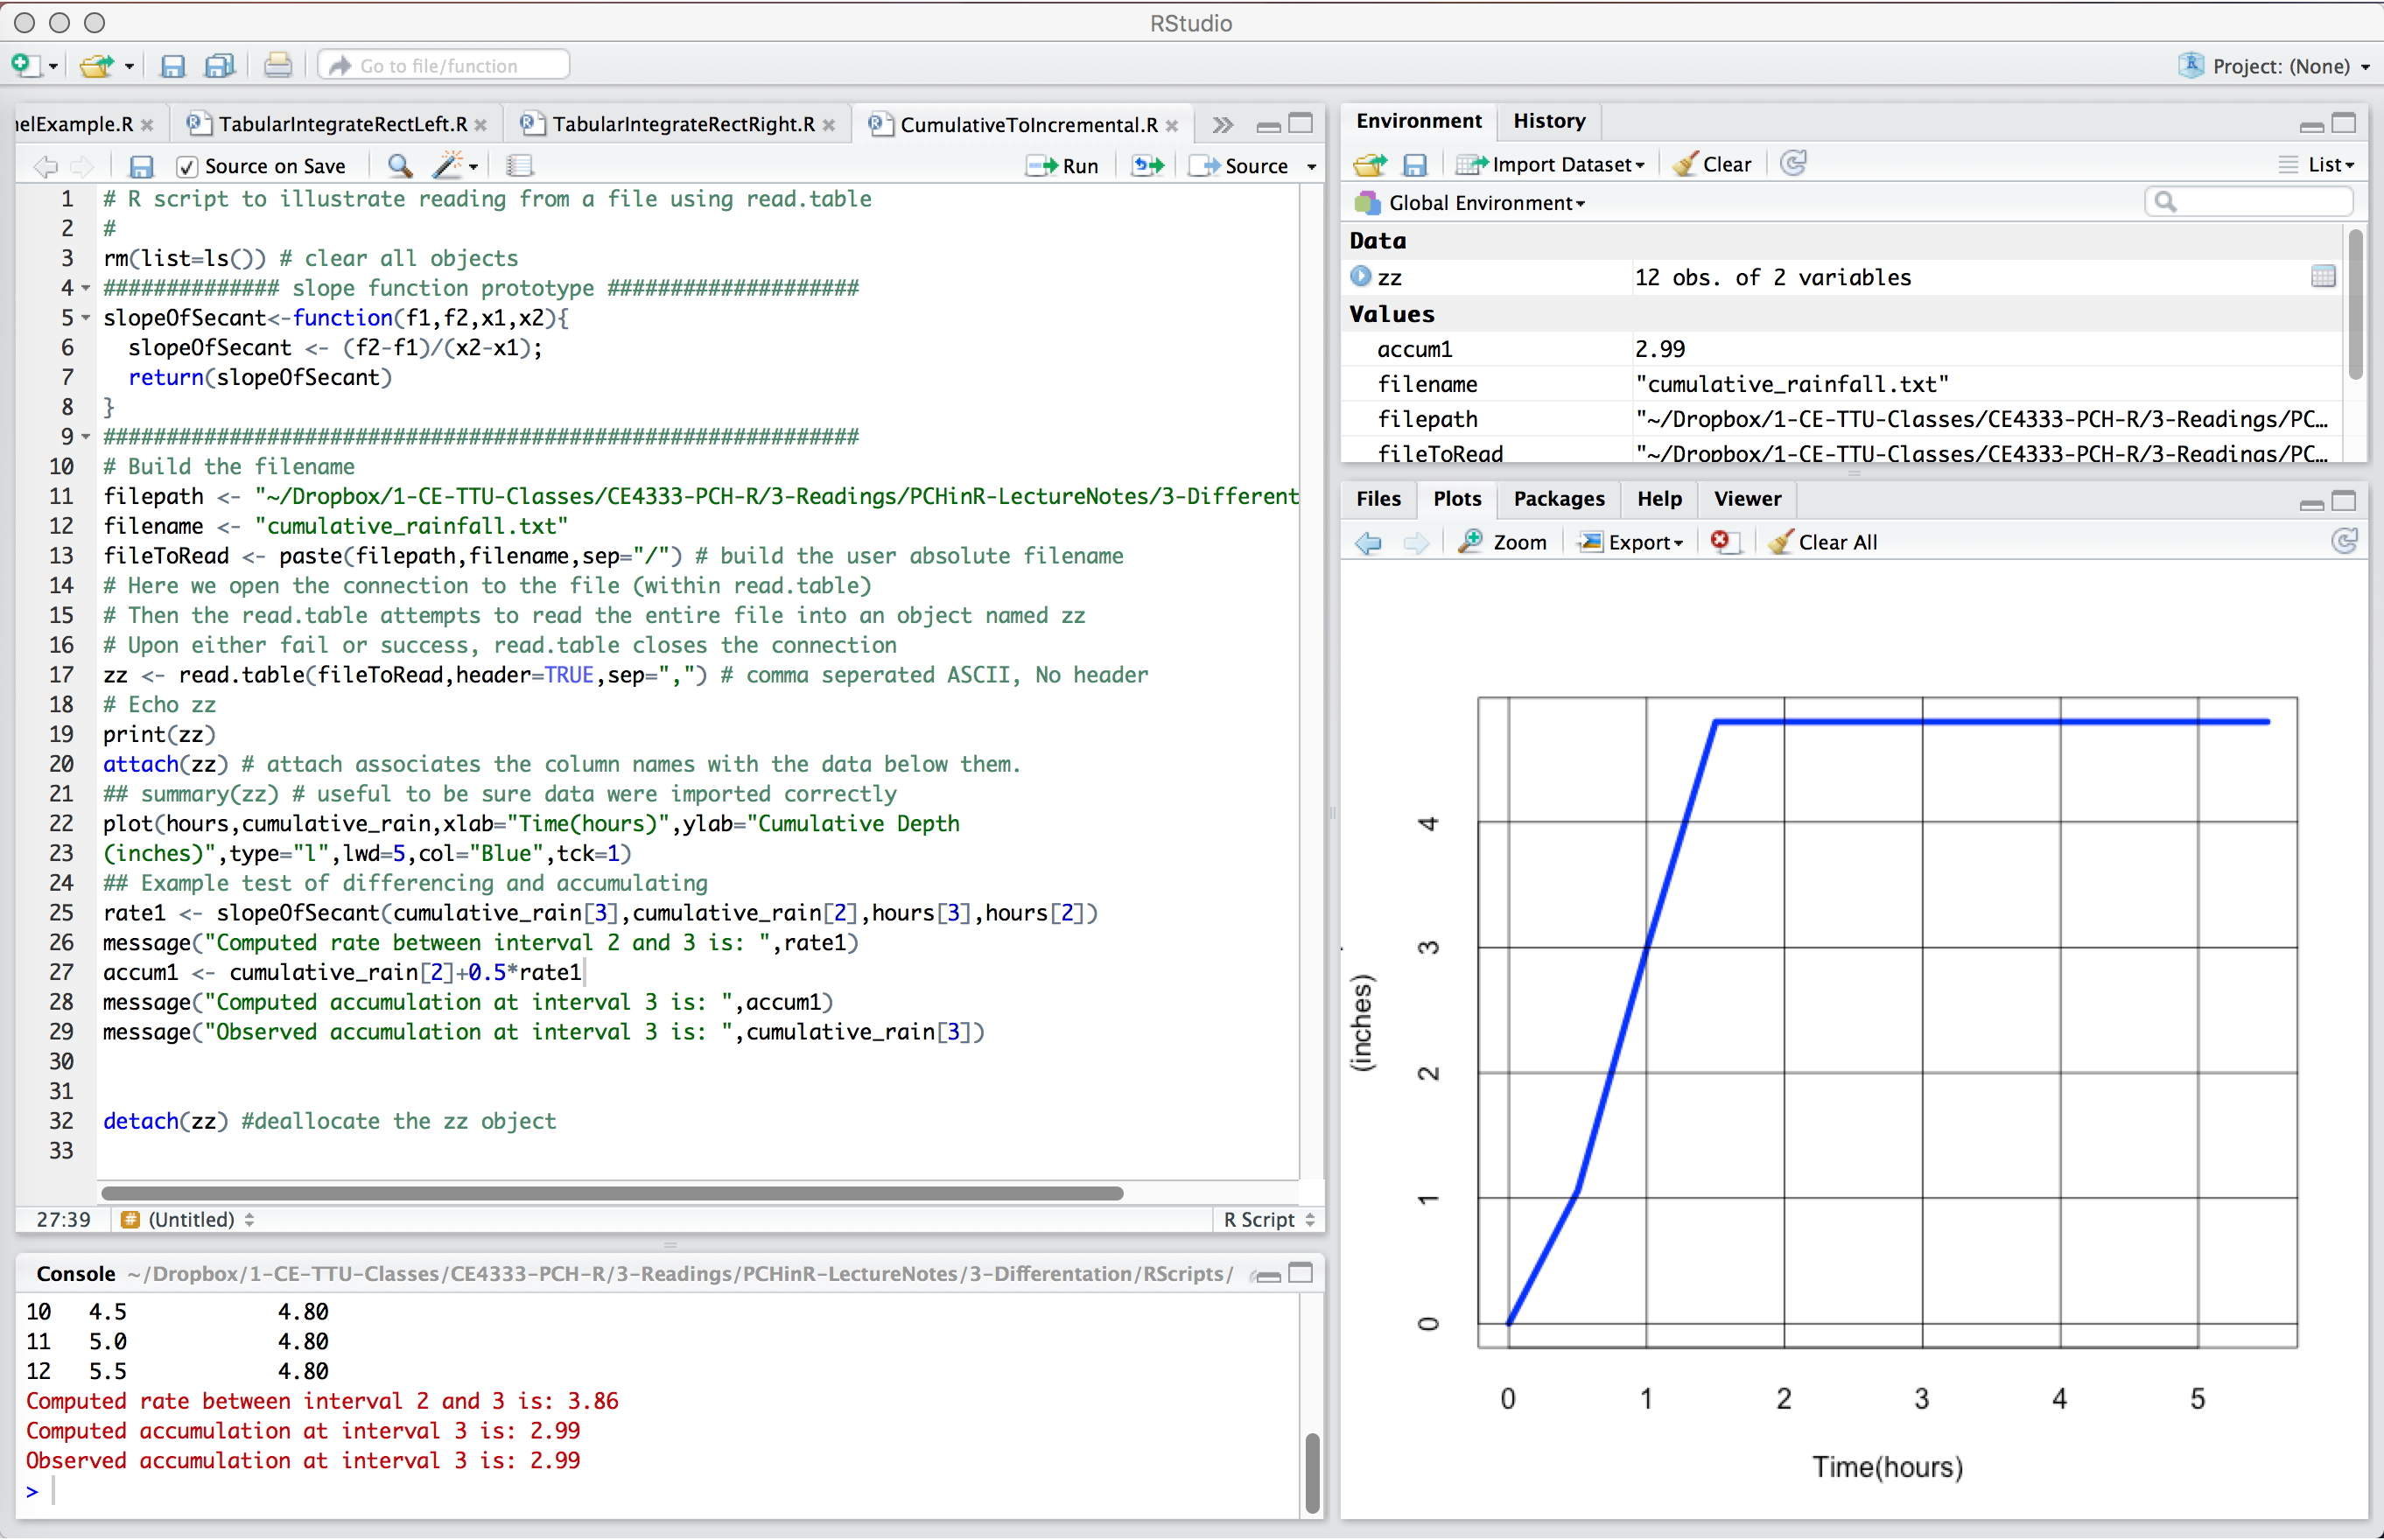
\includegraphics[width=6in]{./3-Differentation/addSecant.jpg} 
   \caption{Script with slopeOfSecant prototype inserted and validation that we recover rate and can re-accumulate correctly}
   \label{fig:addSecant}
\end{figure}

\subsubsection{Disaggregation}
\texttt{disaggregate} is a prototype function that computes the slopes of the secant lines joining adjacent pairs of input data.  Depending on the way the input arrays are presented to the \texttt{disaggregate} function, the function returns either the backward difference approximation to the function's derivative or if an index is presented instead of actual $t$ values, then the function returns the incremental values that when aggregated reconstruct the original input function.

\begin{lstlisting}[caption=R code demonstrating the prototype function \texttt{disaggregate()} , label=lst:Disaggregate]
########      disaggregate function prototype    ###########
# returns a vector of slopes computed by sloepOfSecant 
disaggregate<-function(f,x,dfdx){
  n<-length(x) # length of vectors
  dfdx<-rep(0,n); # zero dfdx
  for (i in 2:n){dfdx[i]<-slopeOfSecant(f[i-1],f[i],x[i-1],x[i]);};
  dfdx[1]<-0;
  return(dfdx)} 
############################################################
\end{lstlisting}

\subsubsection{Numerical Differentiation}

A related concept is to determine the average rate for the time interval, the principal difference is that the rate occurs during the entire time interval and should be assigned to the beginning of the interval instead of the end of the interval.  A subtle change in the \texttt{disaggregate} function can accomplish the task, we will name that new function \texttt{brbt}.  The name is a nemonic for ``backward-rate, backward-time'' differencing.

\begin{lstlisting}[caption=R code demonstrating the prototype function \texttt{brbt()} , label=lst:BrBt]
########### backward rate, backward time prototype ###########
brbt<-function(f,x,dfdx){
  n<-length(x) # length of vectors
  dfdx<-rep(0,n); # zero dfdx
  for (i in 1:(n-1)){dfdx[i]<-slopeOfSecant(f[i],f[i+1],x[i],x[i+1]);};
  dfdx[n]<-0;
  return(dfdx)}
############################################################
\end{lstlisting}

Finally, putting everything together, we have the toolkit to determine the incremental rates (which is an approximation to the derivative of the cumulative rates) and incremental depths which are these individual rates multiplied by the length of the time interval.
Figure \ref{fig:processed_rain_plot} is a screen capture of the \textbf{R} script that implements these functions on the tabular data.

\begin{figure}[h!] %  figure placement: here, top, bottom, or page
   \centering
   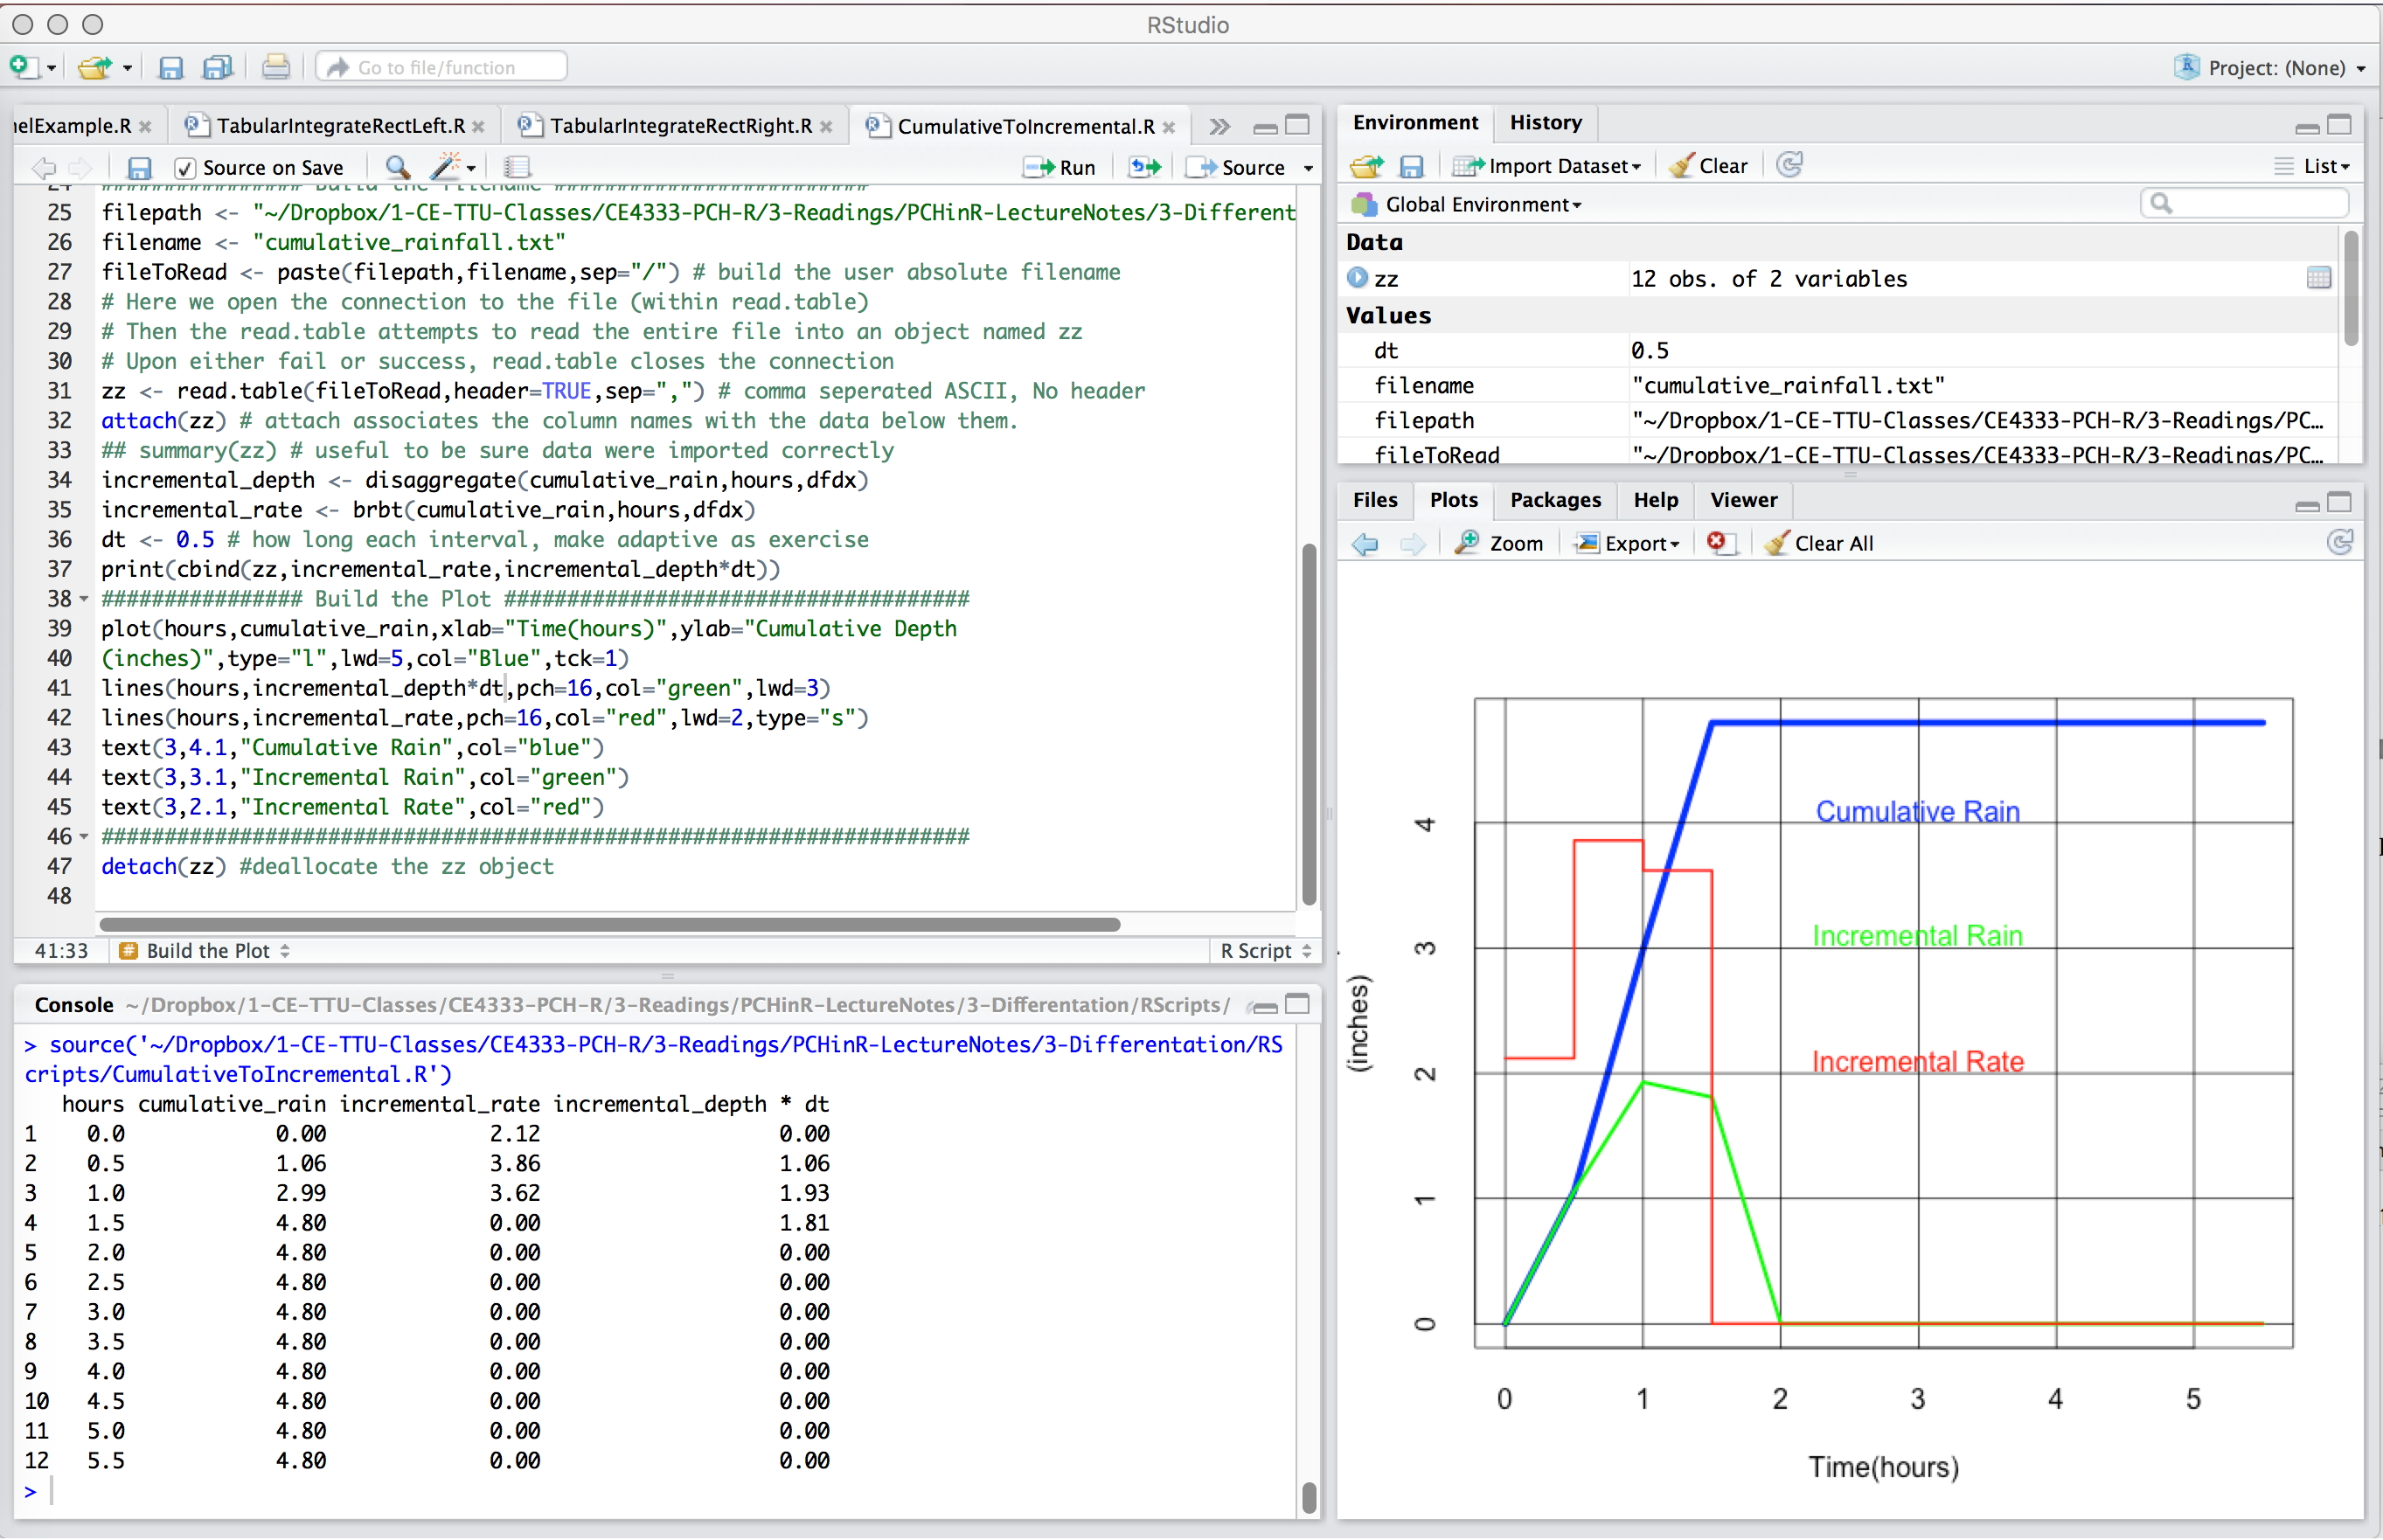
\includegraphics[width=6in]{./3-Differentation/processed_rain_plot.jpg} 
   \caption{Plot of Cumulative Rainfall Time Series (BLUE), Incremental Depth Time Series (GREEN), and Average Rate Time Series (RED)}
   \label{fig:processed_rain_plot}
\end{figure}

Listing \ref{lst:NumDifferencing} is a listing of the \textbf{R} script that produced Figure \ref{fig:processed_rain_plot}.  
The intermediate steps from Figure \ref{fig:addSecant} is removed in this listing.

\begin{lstlisting}[caption=R code demonstrating Numerical Differencing , label=lst:NumDifferencing]
# R script to illustrate numerical differencing 
rm(list=ls()) # clear all objects
############ Prototype (forward define) Functions #########
############## slope function prototype ####################
slopeOfSecant<-function(f1,f2,x1,x2){
  slopeOfSecant <- (f2-f1)/(x2-x1);
  return(slopeOfSecant)}
########      disaggregate function prototype    ###########
disaggregate<-function(f,x,dfdx){
  n<-length(x) # length of vectors
  dfdx<-rep(0,n); # zero dfdx
  for (i in 2:n){dfdx[i]<-slopeOfSecant(f[i-1],f[i],x[i-1],x[i]);};
  dfdx[1]<-0;
  return(dfdx)} 
########### backward rate, backward time prototype ###########
brbt<-function(f,x,dfdx){
  n<-length(x) # length of vectors
  dfdx<-rep(0,n); # zero dfdx
  for (i in 1:(n-1)){dfdx[i]<-slopeOfSecant(f[i],f[i+1],x[i],x[i+1]);};
  dfdx[n]<-0;
  return(dfdx)}
##############################################################

################ Build the filename #########################
filepath <- "~/Dropbox/1-CE-TTU-Classes/CE4333-PCH-R/3-Readings/PCHinR-LectureNotes/3-Differentation/RScripts"
filename <- "cumulative_rainfall.txt"
fileToRead <- paste(filepath,filename,sep="/") # build the user absolute filename
# Here we open the connection to the file (within read.table)
# Then the read.table attempts to read the entire file into an object named zz
# Upon either fail or success, read.table closes the connection
zz <- read.table(fileToRead,header=TRUE,sep=",") # comma seperated ASCII, No header
attach(zz) # attach associates the column names with the data below them.
## summary(zz) # useful to be sure data were imported correctly
incremental_depth <- disaggregate(cumulative_rain,hours,dfdx)
incremental_rate <- brbt(cumulative_rain,hours,dfdx)
dt <- 0.5 # how long each interval, make adaptive as exercise
incremental_depth <- incremental_depth*dt
print(cbind(zz,incremental_rate,incremental_depth))
################ Build the Plot #####################################
plot(hours,cumulative_rain,xlab="Time(hours)",ylab="Cumulative Depth 
(inches)",type="l",lwd=5,col="Blue",tck=1)
lines(hours,incremental_depth*dt,pch=16,col="green",lwd=3)
lines(hours,incremental_rate,pch=16,col="red",lwd=2,type="s")
text(3,4.1,"Cumulative Rain",col="blue")
text(3,3.1,"Incremental Rain",col="green")
text(3,2.1,"Incremental Rate",col="red")
#####################################################################
detach(zz) #deallocate the zz object
\end{lstlisting}

\subsubsection{Aggregation}
Aggregation is the compliment of disaggregation; instead of finding differences we are trying to produce cumulatives from incremental values or rates.  Aggregation is to integration as disaggregation is to differentiation.  Simple aggregation functions are straightforward to build.  Numerical integration (already introduced) is a bit more challenging because there are many different ways to compute areas from tabular data -- we will illustrated rectangular, trapezoidal, and parabolic panels.  

We can insert a prototype \texttt{aggregate} function that simply adds elements in a series to prior elements and stores the value in another series.  Another name for this kind of arithmetic is a running sum.   Functionally, it is rectangular panel (evaluate from the left), numerical integration.
 
\begin{lstlisting}[caption=R code demonstrating the prototype function \texttt{aggregate()} , label=lst:aggregate]
########### aggregate function prototype ###########
aggregate<-function(vector1,vector2){
n<-length(vector1)
# fill vector2 with zeros
vector2<-rep(0,n)
vector2[1]<-vector1[1]+0.0
for(i in 2:n)vector2[i]<-vector2[i-1]+vector1[i]
return(vector2)}
###############################################
\end{lstlisting}

We add this function to the prototype list ate the top of the script and can run
To illustrate the use of \texttt{aggregate} we will aggregate the incremental depths into the cumulative rainfall -- we should recover the original cumulative rainfall series that was originally supplied.

\subsection{Exercises}
\begin{enumerate}
\item Add the \texttt{aggregate} prototype function to collection of prototype functions in the script.
The add some code like:
\begin{verbatim}
new_cum_rain<-aggregate(incremental_depth,dummy)
plot(hours,cumulative_rain,xlab="Time(hours)",ylab="Cumulative Depth
(inches)",type="l",lwd=5,col="Blue",tck=1)
lines(hours,new_cum_rain,col="red",lwd=1.5)
\end{verbatim}
Demonstrate that the two series are identical (e.g. plotting on top of one another).
\item (Advanced) Modify the \texttt{disaggregate()} prototype function to automatically determine the time spacing ($x$) and perform the correct multiplication within the function to return the correct increments.
You only have to add one line of code to the prototype function at
\begin{verbatim}
for (i in 2:n){dfdx[i]<-slopeOfSecant(f[i-1],f[i],x[i-1],x[i]);
	deltax <-   # you need to define this in terms of x[i] and x[i-1]!
	dfdx[i]<- deltax*dfdx[i];};
\end{verbatim}
\end{enumerate}

\subsection{Finite-Difference Formulas}
What we have just done is to explore the use of finite-difference approximations for derivatives. 
Some common formulas for difference formulas are listed below (without derivation -- you should be able to find explanation in any numerical methods text).
All the difference equations presented here are the result of truncated Taylor series expansions about $x$.
The ``order'' refers to the magnitude of truncation error, and this magnitude is proportional to the step size ($\Delta x$) raised to a power (the order).   
Truncation error decreases as the step size is decreased, but one is approaching a divide-by-zero situation (because numerical methods don't do limits just yet!).
\subsubsection{First Derivatives}
Equation \ref{eqn:1st-back} is a first-order backwards difference.
\begin{equation}
\frac{df}{dx} \approx~ \frac{f(x) - f(x -\Delta x)}{\Delta x}
\label{eqn:1st-back}
\end{equation}
Equation \ref{eqn:1st-forward} is a first-order backwards difference.
\begin{equation}
\frac{df}{dx}  \approx~ \frac{f(x + \Delta x) - f(x)}{\Delta x}
\label{eqn:1st-forward}
\end{equation}
Equation \ref{eqn:1st-center} is a second-order central difference.
\begin{equation}
\frac{df}{dx}  \approx~ \frac{f(x + \Delta x) - f(x -\Delta x)}{2 \Delta x}
\label{eqn:1st-center}
\end{equation}
\subsubsection{Second Derivatives}
Equation \ref{eqn:2nd-center} is a second-order central difference.
\begin{equation}
\frac{d^2f}{dx^2}  \approx~ \frac{f(x + \Delta x) - 2f(x) + f(x -\Delta x)}{ \Delta x^2}
\label{eqn:2nd-center}
\end{equation}

\subsubsection{Third Derivatives}
Equation \ref{eqn:3nd-center} is a sixth-order central difference.
\begin{equation}
\frac{d^3f}{dx^3}  \approx~ \frac{f(x + 2\Delta x) -2f(x + \Delta x) + 2f(x -\Delta x) + f(x -2\Delta x)}{ 2 \Delta x^3}
\label{eqn:3nd-center}
\end{equation}

The procedure to generate such difference formulas is general and can supply estimates with approximations of any degree.  
The accuracy depends on the location and number of field variable values involved in the approximation.  
The selection of a formula is not at all trivial (especially with tabulations), but beyond the scope of this handbook.

Despite known complications, this is a general tool used in computational hydraulics and we will use it throughout the remainder of the handbook -- in some examples it will not be obvious that it is finite differencing, and in others it will be explicitly obvious.
The next section introduces Newton's method, and finite-differences will be used to approximate the derivative (Quasi-Newton) to implement the method.  The procedure is really quite common and imbedded in a lot of the computational tools we use professionnaly.
\clearpage

\subsection{Single Variable Quasi-Newton Methods}
%Single variable minimization and root finding are similar numerical exercises.
%Both activities are aimed at finding solutions to the equation $f(x) = 0$, although minimization may not necessarily solve such an equation.\footnote{In essence, root finding can be posed as a minimization problem, but the converse is not true}

The application of fundamental principles of modeling and mechanics often leads to an algebraic or transcendental equation that cannot be easily solved and represented in a closed form.  
In these cases a numerical method is required to obtain an estimate of the root or roots of the expression.  

Newton's method is an iterative technique that can produce good estimates of solutions to such equations.  
The method is employed by rewriting the equation in the form $f(x)=0$, then successively manipulating guesses for $x$ until the function evaluates to a value close enough to zero for the modeler to accept.
  
Figure \ref{fig:ArbitraryFunction} is a graph of some function whose intercept with the $x-$axis is unknown.  
The goal of Newton's method is to find this intersection (root) from a realistic first guess.  
Suppose the first guess is $x_1$, shown on the figure as the right-most specific value of $x$. 
The value of the function at this location is $f(x_1)$.  
Because $x_1$ is supposed to be a root the difference from the value zero represents an error in the estimate.  
Newton's method simply provides a recipe for corrections to this error.  

\begin{figure}[h!] %  figure placement: here, top, bottom, or page
   \centering
   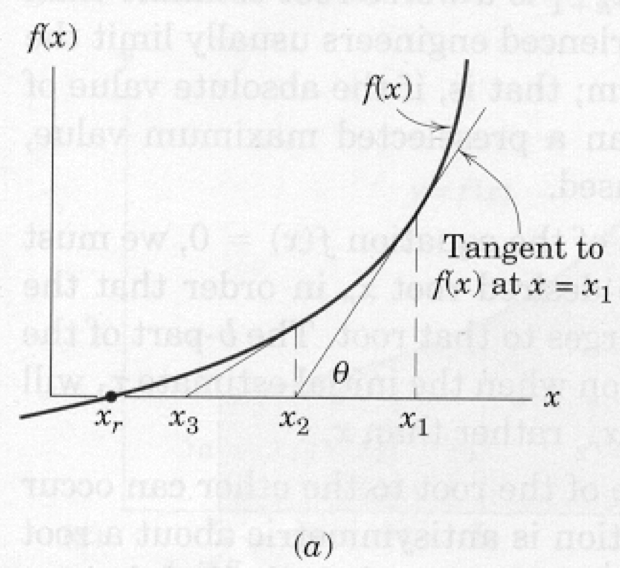
\includegraphics[width=4in]{./3-Differentation/ArbitraryFunction.jpg} 
   \caption{Graph of Arbitrary Function.}
   \label{fig:ArbitraryFunction}
\end{figure}

Provided $x_1$ is not near a minimum or maximum (slope of the function is not zero) then a better estimate of the root can be obtained by extending a tangent line from $x_1,f(x_1)$ to the $x$-axis.  
The intersection of this line with the axis represents a better estimate of the root.

This new estimate is $x_2$.  
A formula for $x_2$ can be derived from the geometry of the triangle $x_2$,$f(x_1)$,$x_1$.   
Recall from calculus that the tangent to a function at a particular point is the first derivative of the function.  
Therefore, from the geometry of the triangle and the definition of tangent we can write,
\begin{equation}
tan(\theta)=\frac{df}{dx}\Biggr\vert_{x_1} = \frac{f(x_1)}{x_1 - x_2}
\end{equation}

Solving the equation for $x_2$ results in a formula that expresses $x_2$ in terms of the first guess plus a correction term.
\begin{equation}
x_2=x_1 - \frac{f(x_1)}{\frac{df}{dx}\vert_{x_1}} 
\end{equation}

The second term on the right hand side is the correction term to the estimate on the right hand side.  
Once $x_2$ is calculated we can repeat the formula substituting $x_2$ for $x_1$ and $x_3$ for $x_2$ in the formula.  
Repeated application usually leads to one of three outcomes:
\begin{enumerate}
\item a root;
\item divergence to $\pm\infty$; or 
\item cycling.
\end{enumerate}

These three outcomes are discussed below in various subsections along with some remedies.


The generalized formula is 

\begin{equation}
x_{k+1}=x_{k} - \frac{  f(x_{k})  }{   \frac{df}{dx}\rvert_{x_k} } 
\label{eqn:NewtonFormula}
\end{equation}

If the derivative is evaluated using analytical derivatives the method is called Newton's method, if approximations to the derivative are used, it is called a quasi-Newton method.

\subsubsection{Newton's Method --- Using analytical derivatives}
This subsection presents an example in \textbf{R} of implementing Newton's method with analytical derivatives.   
The algorithm itself is:
\begin{enumerate}
\item Write the function in proper form, and code it into a computer.
\item Write the derivative in proper form and code it into a computer.
\item Make an initial guess of the solution (0 and 1 are always convenient guesses).
\item Evaluate the function, evaluate the derivative, calculate their ratio.
\item Subtract the ratio from the current guess and save the result as the update.
\item Test for stopping:
\begin{enumerate}
\item Did the update stay the same value? Yes, then stop, probably have a solution.
\item Is the function nearly zero?  Yes, then stop we probably have a solution.
\item Have we tried too many updates? Yes, then stop the process is probably cycling, stop.
\end{enumerate}
\item If stopping is indicated proceed to next step, otherwise proceed back to step 4.
\item Stopping indicated, report last update as the result (or report failure to find solution), and related information about the status of the numerical method.
\end{enumerate}

The following example illustrates these step as well as a \textbf{R} implementation of Newton's method.

Suppose we wish to find a root (value of $x$) that satisfies Equation \ref{eqn:FindARoot}.
\begin{equation}
f(x) = e^x - 10 cos(x) -100
\label{eqn:FindARoot}
\end{equation}

Then we will need to code it into a script.   Here is a code fragment that will work:
\begin{lstlisting}[caption=R code fragment for the function calculation, label=lst:NewtonsFunction]
# Define Function Here
func <- function(x)
{
  func <- exp(x)-10*cos(x)-100;
  return(func);
}
\end{lstlisting}

%Notice in the code fragment we import three built-in functions from the \textbf{Python} \texttt{math} package, specifically $\exp()$, $\sin()$, and $\cos ()$.

The next step is to code the derivative.   In this case, Equation \ref{eqn:DerFind} is the derivative of Equation \ref{eqn:FindARoot}.

\begin{equation}
\frac{df}{dx}\vert{(x)} = e^x + 10 \sin(x)
\label{eqn:DerFind}
\end{equation}

A code fragment to compute the value of the derivative at any value of $x$ that will work is:

\begin{lstlisting}[caption=R code fragment for the derivative calculation, label=lst:NewtonsDerivative]
# Define Derivative Here
dfdx <- function(x)
{
  dfdx <- exp(x) + 10*sin(x); 
  return(dfdx);
}
\end{lstlisting}

Next we will need script to read in an initial guess, and ask us how many trials we will use to try to find a solution, as well as how close to zero we should be before we declare victory.   
\newpage

\begin{lstlisting}[caption=R code fragment for reading input data from the programmer, label=lst:InputNewtonData]
# Read some values from the console
message('Enter an initial guess for X for Newton method :  ')
xnow <- as.numeric(readline())
message('Enter iteration maximum :  ')
HowMany <- as.numeric(readline())
message('Enter a tolerance value for stopping (e.g. 1e-06) :  ')
HowSmall <- as.numeric(readline())
## There are several other ways to make these reads!  The scan() function would probably also work.
\end{lstlisting}



The use of \texttt{HowSmall}; is called a zero tolerance.   We will use the same numerical value for two tolerance tests.   Also notice how we are using error traps to force numeric input.   Probably overkill for this example, but we already wrote the code in an earlier chapter, so might as well use the code.  Professional codes do a lot of error checking before launching into the actual processing --- especially of the processing part is time consuming, its worth the time to check for obvious errors before running far a few hours then at some point failing because of an input value error that was predictable.

Now back to the tolerance tests. The first test is to determine if the update has changed or not.   If it has not, we may not have a correct answer, but there is no point continuing because the update is unlikely to move further.   The test is something like

\begin{math}
\text{IF}~\lvert x_{k+1} - x_{k} \rvert < \text{Tol.~ THEN Exit and Report Results}
\end{math}  

The second test is if the function value is close to zero.   The structure of the test is similar, just an different argument.   The second test is something like

\begin{math}
\text{IF}~\lvert f(x_{k+1}) \rvert < \text{Tol.~ THEN Exit and Report Results}
\end{math} 

One can see from the nature of the two tests that a programmer might want to make the tolerance values different.   This modification is left as a reader exercise.

Checking for maximum iterations is relatively easy, we just include code that checks for normal exit the loop.\footnote{Rather than breaking from the loop.}

Now we simply connect the three fragments, and we have a working \textbf{R} script that implements Newton's method for Equation \ref{eqn:FindARoot}.  
Listing \ref{lst:NewtonsMethod} is the entire code module that implements the method, makes the various tests, and reports results.
Figure \ref{fig:NewtonTrials} is a screen capture of the program run in \textbf{R}.

The example is specific to the particular function provided, but the programmer could move the two functions \texttt{func} and \texttt{dfdx} into a user specified module, and then load that module in the program to make it even more generic.   The next section will use such an approach to illustrate the ability to build a generalized Newton method and only have to program the function itself.

\newpage
\begin{lstlisting}[caption=R code demonstrating Newton's Method calculations, label=lst:NewtonsMethod]
# Newtons Method in R
# Define Function Here
func <- function(x)
{
  func <- exp(x)-10*cos(x)-100;
  return(func);
}
# Define Derivative Here
dfdx <- function(x)
{
  dfdx <- exp(x) + 10*sin(x); 
  return(dfdx);
}
# Newton's Method Here
# Read some values from the console
message('Enter an initial guess for X for Newton method :  ')
xnow <- as.numeric(readline())
message('Enter iteration maximum :  ')
HowMany <- as.numeric(readline())
message('Enter a tolerance value for stopping (e.g. 1e-06) :  ')
HowSmall <- as.numeric(readline())
# Now start the iterations
for (i in 1:HowMany) {
  xnew <- xnow - func(xnow)/dfdx(xnow)
# test for stopping
  if (abs(xnew-xnow) < HowSmall){
    message('Update not changing')
    xnow <- xnew
    print(cbind(xnow,xnew,func(xnew)))
    break
  }
  if (abs(func(xnew) < HowSmall)) {
    message('Function value close to zero')
    xnow <- xnew
    print(cbind(xnow,xnew,func(xnew)))
    break    
  }
# next iteration
xnow <- xnew
}
if (i >= HowMany){
  message('Iteration limit reached')
  print(cbind(xnow,xnew,func(xnew)))
}
\end{lstlisting}

\begin{figure}[h!] %  figure placement: here, top, bottom, or page
   \centering
   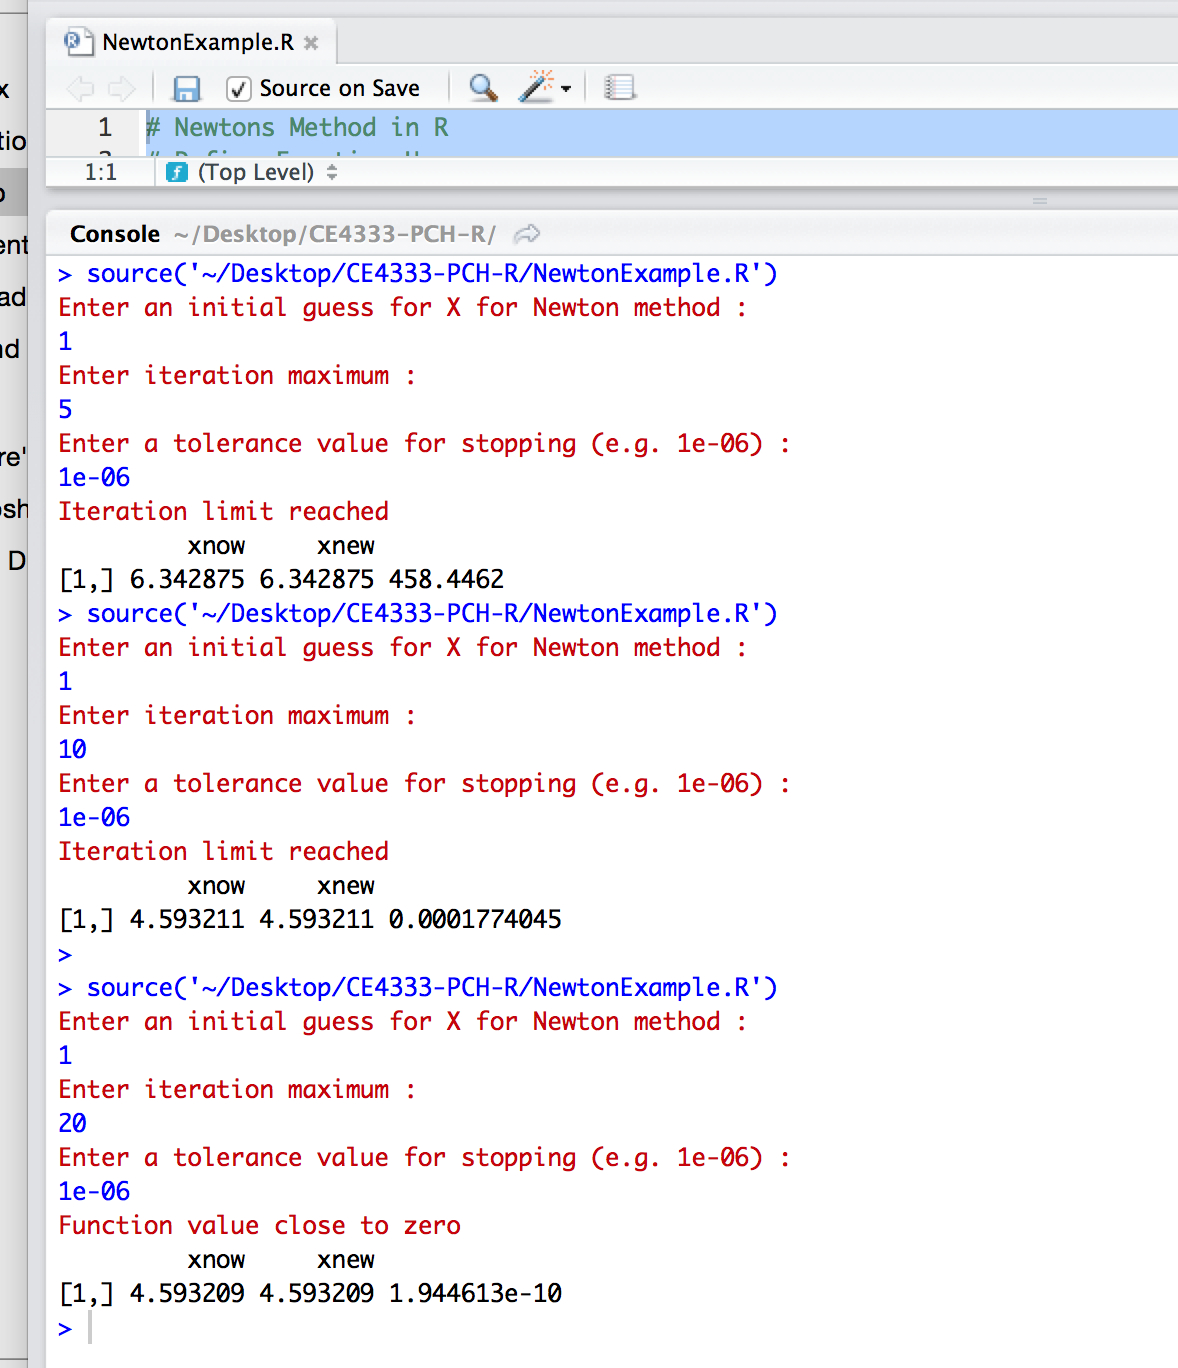
\includegraphics[width=6in]{./3-Differentation/NewtonTrials.jpg} 
   \caption{Several runs of the program using the analytical derivative to illustrate different kinds of responses.}
   \label{fig:NewtonTrials}
\end{figure}

%%%%%%%%%%%%%%%%%%%%%%%%%%%%%%%%%%%%%%%%
\subsubsection{Newton's Method --- Using Finite-Differences to estimate derivatives}
A practical difficulty in using Newton's method is determining the value of the derivative in cases where differentiation is difficult.  
In these cases we can replace the derivative by a difference equation and then proceed as in Newton's method. 

Recall from calculus that the derivative was defined as the limit of the difference quotient:
\begin{equation}
\frac{df}{dx}\vert_{x} = \lim_{\Delta x \rightarrow 0}\frac{f(x + \Delta x) - f(x) }{\Delta x}
\end{equation}

A good approximation to the derivative should be possible by using this formula with a small, but non-zero value for $\Delta x$.

\begin{equation}
\frac{df}{dx}\vert_{x} \approx \frac{f(x + \Delta x) - f(x) }{\Delta x}
\end{equation}

When one replaces the derivative with the difference formula the root finding method the resulting update formula is

\begin{equation}
x_{k+1}=x_k - \frac{f(x_k) \Delta x}{f(x_k + \Delta x)-f(x_k)} 
\label{eqn:QuasiNewtonFormula}
\end{equation}

This root-finding method is called a quasi-Newton method.

Listing \ref{lst:QNewton}  is the code fragment that we change by commenting out the analytical derivative and replacing it with a first-order finite difference approximation of the derivative.  
The numerical value $1e-06$ is called the step size ($\Delta x$)  and should be an input value (rather than built-in to the code as shown here) like the tolerance test values, and be passed to the function as another argument.

\begin{lstlisting}[caption=R code demonstrating Newton's Method calculations, label=lst:QNewton]
# Define Derivative Here
dfdx <- function(x)
{
#  dfdx <- exp(x) + 10*sin(x); 
    dfdx <- (func(x + 1e-06) - func(x) )/ (1e-06);
# func must already exist before first call!
  return(dfdx);
}
\end{lstlisting}

Starting with the last example lets modify the analytical version of the code by inserting the above fragment in place of the analytical derivative.  Listing \ref{lst:QuasiNewton} is the listing with the modification in place.  Notice we have only changed a single line, and not have a more flexible tool.  The next modification (left as an exercise) is to detach the creation of the function from the main algorithm, then we would have a general purpose Quasi-Newton's method.

\begin{lstlisting}[caption=R code demonstrating Newton's Method calculations using finite-difference approximation for the derivative, label=lst:QuasiNewton]
# Newtons Method in R
# Define Function Here
func <- function(x)
{
  func <- exp(x)-10*cos(x)-100;
  return(func);
}
# Define Derivative Here
dfdx <- function(x)
{
#  dfdx <- exp(x) + 10*sin(x); 
  dfdx <- (func(x + 1.0e-06) - func(x))/(1.0e-06)
  return(dfdx);
}
# Newton's Method Here
# Read some values from the console
message('Enter an initial guess for X for Newton method :  ')
xnow <- as.numeric(readline())
message('Enter iteration maximum :  ')
HowMany <- as.numeric(readline())
message('Enter a tolerance value for stopping (e.g. 1e-06) :  ')
HowSmall <- as.numeric(readline())
# Now start the iterations
for (i in 1:HowMany) {
  xnew <- xnow - func(xnow)/dfdx(xnow)
# test for stopping
  if (abs(xnew-xnow) < HowSmall){
    message('Update not changing')
    xnow <- xnew
    print(cbind(xnow,xnew,func(xnew)))
    break
  }
  if (abs(func(xnew) < HowSmall)) {
    message('Function value close to zero')
    xnow <- xnew
    print(cbind(xnow,xnew,func(xnew)))
    break    
  }
# next iteration
xnow <- xnew
}
if (i >= HowMany){
  message('Iteration limit reached')
  print(cbind(xnow,xnew,func(xnew)))
}
\end{lstlisting}



Listing \ref{lst:QuasiNewton} is the main code.  Notice how the function definitions are changed, in particular \texttt{dfdx}.



Figure \ref{fig:NewtonTrials2} is a screen capture of the program run after the code modification above.   
\begin{figure}[h!] %  figure placement: here, top, bottom, or page
   \centering
   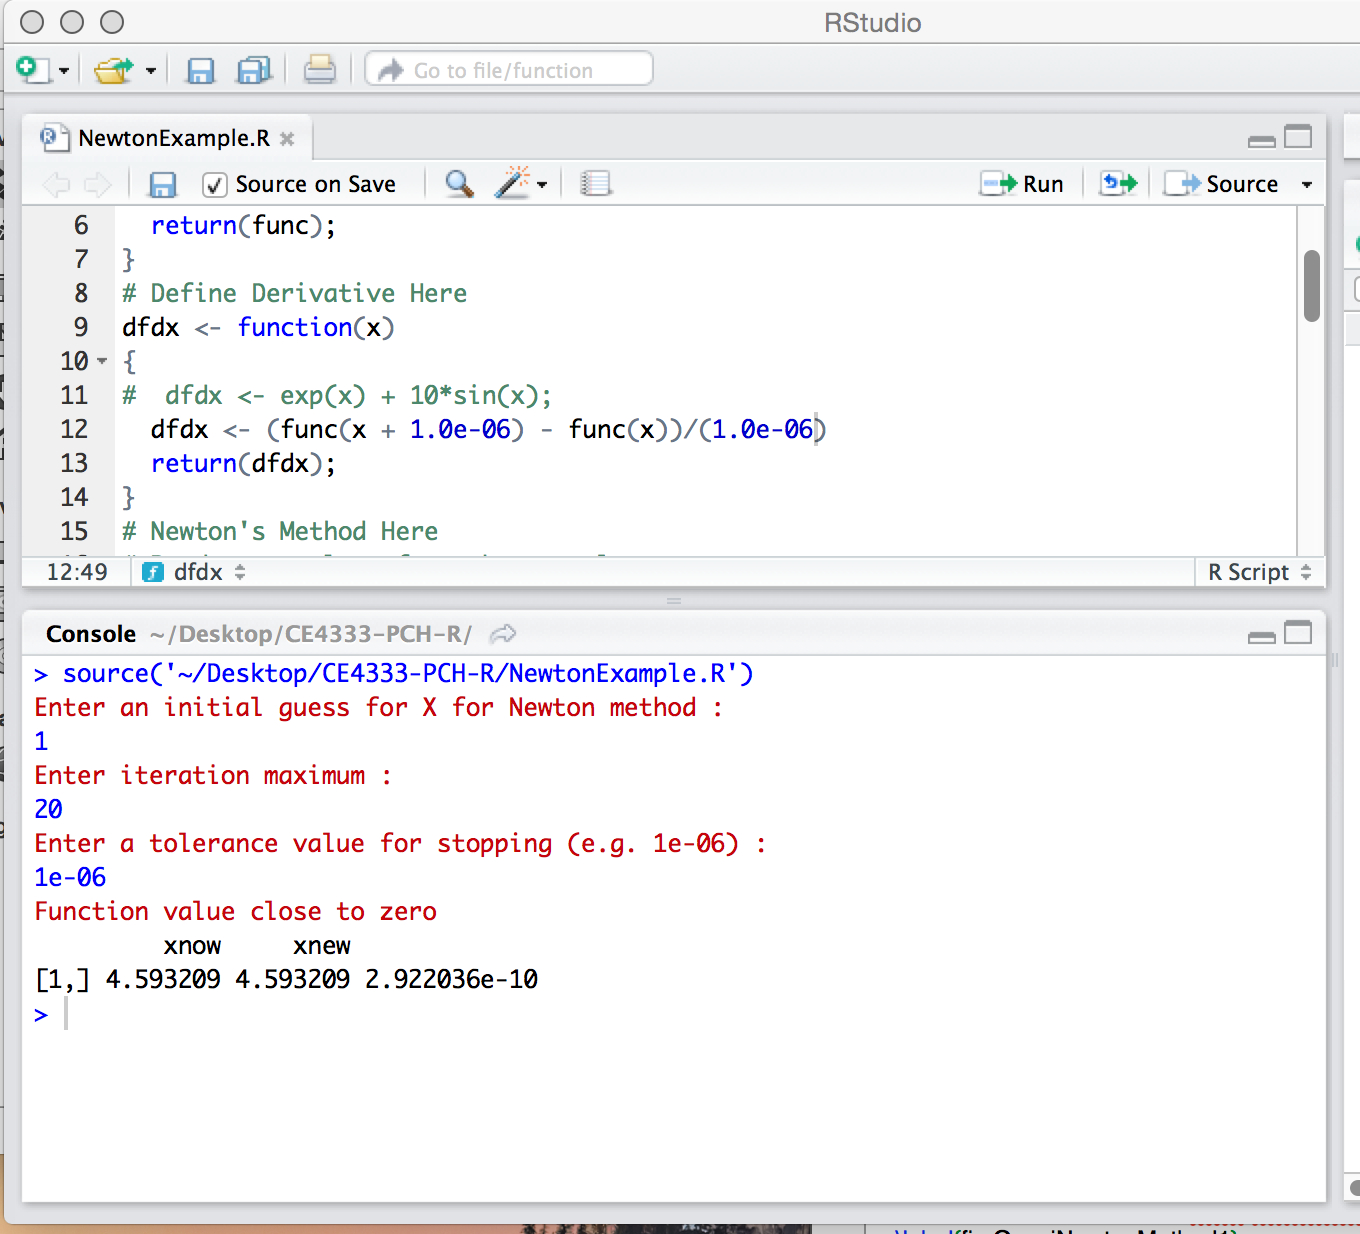
\includegraphics[width=6in]{./3-Differentation/NewtonTrials2.jpg} 
   \caption{Program run after changing from analytical to finite-difference approximation for the derivative.}
   \label{fig:NewtonTrials2}
\end{figure}

The~advantage of the approximate derivative is that we don't have to do the calculus --- just code in the function.  

The obvious advantage of modular coding is to protect the parts of the code that are static, and just modify the function definitions.   We can keep a working example around in case we break something and use that to find what we broke.

\subsubsection{Method Fails}
The three subsections below describe the ways that the method routinely fails, along with some suggestions for remedy.   Generally we should plot the function before trying to find a root, but sometimes the root finding is a component of a more complex program and we just want it to work.   In that situation, the programmer would build in many more tests that the three above to try to force a result before giving up.   
\subsubsection{Multiple Roots}
Figure \ref{fig:MultipleRoots} illustrates the behavior in the presence of multiple roots.  
When there are multiple roots the method will converge on the root that that is defined by the initial guess.\footnote{This behavior is called ``sensitive dependence on initial conditions''.}  
The initial estimate must be close enough to the desired root to converge to the root.\footnote{Ironically, we need a good idea of the answer before we start the method.}
\begin{figure}[h!] %  figure placement: here, top, bottom, or page
   \centering
   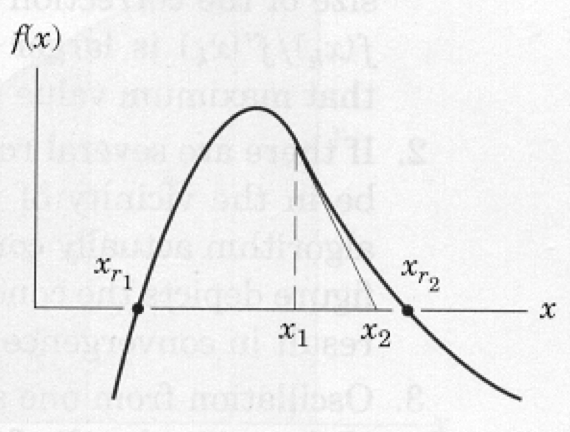
\includegraphics[width=4in]{./3-Differentation/MultipleRoots.jpg} 
   \caption{Multiple roots.}
   \label{fig:MultipleRoots}
\end{figure}
Another challenge is what happens if the initial guess is at the divide (the peak of the function in Figure \ref{fig:MultipleRoots}); in such cases we may actually get a divergent solution because the slope of the function at that peak is nearly zero.  
\subsubsection{Cycling}
Cycling can occur when the root is close to an inflection point of the function.  
Usual practice is to again limit the step size to prevent such behavior.  
Figure \ref{fig:RootCycling} is an illustration of cycling.
\begin{figure}[h!] %  figure placement: here, top, bottom, or page
   \centering
   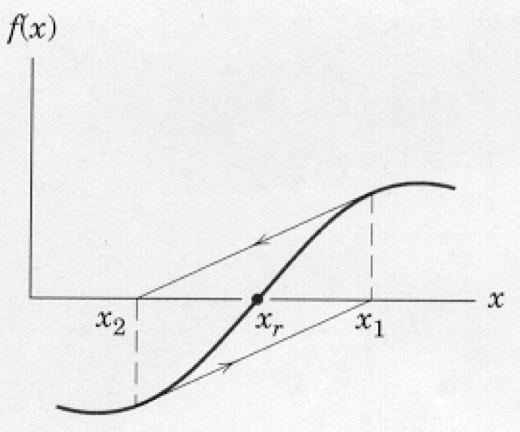
\includegraphics[width=4in]{./3-Differentation/RootCycling.jpg} 
   \caption{Estimates cycling around a root.}
   \label{fig:RootCycling}
\end{figure}
A good remedy for cycling is to first detect the cycling, then provide a small ``shove'' to the guess.  
Examination of root finding codes often reveals a pseudo-random number generator within the code that will provide this shove when cycling is detected.
\subsubsection{Near-zero derivatives}
The derivative in Equation \ref{eqn:NewtonFormula} must not be zero, otherwise the guess corresponds to a maximum or minimum of the function and the tangent line will never intersect the x-axis.    
The derivative must not be too close to zero, otherwise the slope will be so small as to make the correction too large to produce a meaningful update.  Usual practice is to limit the size of the correction term to some maximum and to use this maximum value whenever the formula prescribes a larger step.
Divergence to $\pm\infty$ is usually explained by near-zero derivatives at the sign change. 
The bi-section method is a little more robust in this respect.
\subsection{Related Concepts}
A couple of other root finding methods are worth mentioning because they can sometimes serve as a fallback when Newton's method fails.   Two robust methods are bisection and false-positioning. These are discussed in the suggested reading list in Chapra's textbook.
%\subsubsection{Root finding by bisection}
%\subsubsection{Root finding by false-positioning}

\clearpage
\subsection{Exercise Set 3}
\begin{enumerate}
\item Build a Newton's Method program (or use mine) and make the program request a tolerance value for ``how close to zero'' is the function, and ``how small is the change in update values.''  Build your code using the modular approach (two files).  Test your code using the same example in the notes.

\item Now modify the main and the function module to use approximate derivatives (the finite-difference formulation) and require the user supply a step size.   Test the code using the same example in the notes.

For each of the exercises above, prepare documentation similar to the notes where you describe the salient points of your program.   

\item  Now use your program to find roots for the following equations:
\begin{enumerate}
\item $\exp(x) - 3x^2 =0$ \\
\item $\ln(x) - x + 2 = 0$ \\
\item $\tan(x) - x - 1 = 0$ \\
\end{enumerate}
For these three equations, document your search for roots.  Identify if there are bad initial guesses that cause the program to fail to find a root.   Also the equations may have multiple roots.  If you discover multiple roots, identify the starting values one needs to use to converge to a particular root.


\end{enumerate}

These exercises are also located on the class server in \texttt{ES-3}.
%%%%%%%%%%%%%%%%%%%%%%%%%%%%%%%%%%%%%%%%%%%%%%%%%%%%%%%%%%%%%
%%%%%%%%%%%%%%%%%%%%%%%%%%%%%%%%%%%%%%%%%%%%%%%%%%%%%%%%%%%%%%

